\documentclass[11pt,a4paper]{article}

\usepackage[utf8]{inputenc}
\usepackage[T1]{fontenc}
\usepackage[english]{babel}
\usepackage{lmodern}
\usepackage{microtype}
\usepackage[a4paper,margin=2.5cm]{geometry}
\usepackage{amsmath,amssymb,amsfonts,bm,mathtools}
\usepackage{amsthm}
\usepackage{booktabs,array}
\usepackage{graphicx}
\usepackage{float}
\usepackage[section]{placeins}
\usepackage{subcaption}
\usepackage{pgfplots}
\usepgfplotslibrary{groupplots}
\pgfplotsset{compat=1.18}
\usepackage{xcolor,xurl}
\usepackage[colorlinks=true,
  linkcolor=blue,
  citecolor=blue,
  urlcolor=blue,
  pdfborder={0 0 0},
  pdftitle={Relational Capacity Dynamics, RFG, and the RFG-R Effective Completion},
  pdfauthor={Martin Petrásek},
  pdfsubject={Relational Capacity Dynamics and Relational Foliation Gravity},
  pdfkeywords={relational capacity, preferred foliation, modified gravity, cosmology, gravitational waves, standard sirens}]{hyperref}
\usepackage{enumitem}
\usepackage{physics}
\setlength{\parindent}{1.1em}
\setlength{\parskip}{0.3em}
\setlength{\emergencystretch}{3em}
\renewcommand{\arraystretch}{1.15}

\newtheorem{axiom}{Axiom}[section]
\newtheorem{definition}[axiom]{Definition}
\newtheorem{theorem}[axiom]{Theorem}
\newtheorem{lemma}[axiom]{Lemma}
\newtheorem{proposition}[axiom]{Proposition}
\newtheorem{corollary}[axiom]{Corollary}
\newtheorem{remark}[axiom]{Remark}
\newtheorem{openproblem}[axiom]{Open problem}

\newcommand{\C}{\mathcal{C}}
\newcommand{\Cs}{\mathcal{C}_\star}
\newcommand{\Jc}{\mathbf{J}_{\mathcal{C}}}
\newcommand{\Sc}{\mathcal{S}_{\mathcal{C}}}
\newcommand{\Ac}{\mathbf{A}_{\mathcal{C}}}
\renewcommand{\dd}{\mathrm{d}}
\newcommand{\e}{\mathrm{e}}
\newcommand{\Lag}{\mathcal{L}}
\newcommand{\Ham}{\mathcal{H}}
\newcommand{\RCD}{\mathrm{RCD}}
\newcommand{\RFG}{\mathrm{RFG}}
\newcommand{\rhoC}{\rho_{\mathcal{C}}}
\newcommand{\kC}{\kappa_{\mathcal{C}}}
\newcommand{\mpl}{M_{\rm Pl}}
\newcommand{\threeR}{{}^{(3)}R}
% Permanent public source location; the complete local bundle is nested below.
\newcommand{\RFGRepoURL}{https://github.com/MartinPetrasek123/MartinPetrasek123}
\newcommand{\RFGRepoPath}[1]{\href{\RFGRepoURL/tree/main/r-universe-complete-chain/rfg-r-completion/r_universe_completion/#1}{\texttt{#1}}}
\newcommand{\RFGLocalPath}[1]{\texttt{r\_universe\_completion/#1}}
% note: keep single outer brace group for safe use inside \bigl( ... \bigr)
\newcommand{\Boxed}[1]{\boxed{\displaystyle #1}}
\newcommand{\doi}[1]{\href{https://doi.org/#1}{\textcolor{blue}{doi:#1}}}

\title{\textbf{Relational Capacity Dynamics, Relational Foliation Gravity, and RFG-R}\\[0.4em]
\large Full proof version: original branch, regular effective completion,\\ local-GR matching, and a reproducible matter/CMB likelihood specification}

\author{Martin Petr\'{a}sek\\[0.3em]
\small ORCID: \href{https://orcid.org/0009-0007-4512-9528}{0009-0007-4512-9528}\\[0.2em]
\small Institute for Resonant Synthesis and Field Physics (IRSFP)\\
\small Prague, Czech Republic\\
\small \href{mailto:martin.petrasek@irsfp.org}{martin.petrasek@irsfp.org}}

\date{July 2026}

\begin{document}

\maketitle

\begin{abstract}
We present a unified theoretical framework that begins with a non-geometric macroscopic scalar theory---Relational Capacity Dynamics (RCD)---and constructs a covariant preferred-foliation completion---Relational Foliation Gravity (RFG). The primitive variable of the scalar sector is a strictly positive relational-capacity field \(\C(\tau,\mathbf{x})\). We supply the complete ontology, dimensional structure, conservative action, full variational derivation, Hamiltonian formulation, Noether identities with explicit local currents, finite-response transport, emergent physical-time map, and linear stability analysis. The scalar sector is ghost-free for \(\rhoC>0\), gradient-stable for \(\kC>0\), and strictly hyperbolic with characteristic speed \(c_{\mathcal{C}}=\sqrt{\kC/\rhoC}\).

The original covariant completion is defined by a metric--khronon action whose two free functions are uniquely reconstructed from a conserved relational-capacity law and the requirement of luminal tensor propagation. The resulting homogeneous cosmology yields the closed algebraic equation
\[
E^2=\Omega_{m0}a^{-3}+\Omega_{r0}a^{-4}+\Omega_{R0}E^{2-\theta},
\]
together with a proof of existence and uniqueness of the expanding branch, exact expressions for the logarithmic Hubble derivative, deceleration parameter, effective equation of state, acceleration--capacity identity, early- and late-time asymptotics, and a falsifiable standard-siren distance relation with \(c_T=1\).

The RFG-R extension introduced here is a separate, explicitly defined low-energy multiscale EFT. It regularizes the \(X\to0\) action, preserves the original homogeneous branch to controlled order, and matches exactly to GR in a specified local-curvature domain. It consequently gives a definite local PPN prediction. Its regularized action, potential reconstruction, numerical validation, and Cassini likelihood factor are supplied as executable source files. The matter/CMB contribution is a full-spectrum Einstein--Boltzmann likelihood emph{specification}, with fixed inputs, stability rejections, and outputs; no CMB likelihood has yet been run. The original RFG scalar linearization degeneracy and the absence of a completed matter-coupled scalar reduction are retained as limitations, not hidden by the RFG-R definition. No claim is made that either construction has displaced \(\Lambda\)CDM.
\end{abstract}

\bigskip
\noindent\textbf{Keywords:}
Relational Capacity Dynamics (RCD);
Relational Foliation Gravity (RFG);
emergent time;
relational capacity;
preferred foliation;
scalar field theory;
modified gravity;
Hamiltonian formulation;
Noether currents;
hyperbolic field equations;
cosmology;
gravitational waves;
standard sirens.

\newpage
\section{Introduction}

A fundamental theory must specify its dynamical variables, symmetries, action, variational equations, physical degrees of freedom, initial-value structure, and falsification conditions. A background equation alone is not sufficient. The purpose of this manuscript is to assemble the mathematically derived RCD and RFG layers together with a deliberately explicit, regular low-energy extension, RFG-R. The distinction is essential: RFG-R is a model completion and matching prescription, not a retroactive theorem about the original singular RFG branch.

We distinguish three logically separate statements that must not be conflated:

\begin{enumerate}[label=(\roman*)]
\item \textbf{Mathematical definition:} the action and its variational problem are specified.
\item \textbf{Internal viability:} all propagating modes must be ghost-free, gradient-stable, and compatible with a well-posed initial-value problem.
\item \textbf{Empirical viability:} cosmological, Solar-System, binary-pulsar, gravitational-wave and laboratory data must be fitted with a reproducible likelihood.
\end{enumerate}

The original calculation completes item~(i) for the scalar macroscopic sector and for the homogeneous and tensor sectors of the preferred-foliation theory. RFG-R additionally defines a regular action and an exact local-GR domain, but it does not make the original scalar perturbation degeneracy disappear. Preferred-foliation and ADM-based constructions provide the broader mathematical context~\cite{ADM,JacobsonMattingly,Horava,BlasPujolasSibiryakov}. The likelihood protocol uses a full 3+1 EFT Einstein--Boltzmann backend rather than a background-only surrogate~\cite{EFTCAMB,HEFTCAMB}.

The logical hierarchy followed throughout is
\[
\text{ontology}\;\longrightarrow\;
\text{state space}\;\longrightarrow\;
\text{action}\;\longrightarrow\;
\text{equations}\;\longrightarrow\;
\text{stability}\;\longrightarrow\;
\text{observables}.
\]

\begin{table}[H]
\centering
\caption{Scope comparison for the constructions in this paper. ``Defined'' is not a data fit, and an entry for a particular sector does not imply health of every perturbative sector.}
\label{tab:comparison}
\resizebox{\textwidth}{!}{%
\begin{tabular}{@{}lcccc@{}}
\toprule
Framework & Scalar status & Tensor speed & Effective \(w_R(a)\) & Analytic background closure \\
\midrule
\(\Lambda\)CDM & N/A & \(c_T=1\) & \(w=-1\) (const.) & Yes \\
Quintessence / K-essence & Conditional (\(c_s^2>0\)) & \(c_T=1\) & Potential-dependent & Selected potentials only \\
Horndeski / DHOST & After cleaning & Generally \(c_T(z)\neq1\) & Dynamical & Varies \\
\textbf{RCD / original RFG} & RCD stable; RFG FLRW scalar degeneracy & \(c_T=1\) (exact) & \(w_R(a)>-1\) (derived) & Yes (Eq.~\eqref{eq:background}) \\
\textbf{RFG-R EFT} & Matter scalar not yet reduced & \(c_T=1\) on FLRW & Regularized branch & Yes (Eq.~\eqref{eq:RFGR-background}) \\
\bottomrule
\end{tabular}%
}
\end{table}

\begin{table}[H]
\centering
\caption{Closure ledger used throughout the manuscript. The table prevents a common failure mode in speculative theory papers: treating a selected branch, reconstruction condition, or calculational target as if it were already a theorem.}
\label{tab:closure-ledger}
\resizebox{\textwidth}{!}{%
\begin{tabular}{@{}p{0.23\textwidth}p{0.25\textwidth}p{0.42\textwidth}@{}}
\toprule
Layer & Status in this manuscript & Precise content \\
\midrule
RCD scalar ontology and action & Closed classical sector & \(\C>0\), \(\varphi=\ln(\C/\Cs)\), action, Euler--Lagrange equation, Hamiltonian, Noether currents, linear hyperbolicity. \\
Finite-response transport & Closed once constitutive data are fixed & Maxwell--Cattaneo relaxation law and entropy-production condition; not a fundamental microscopic derivation. \\
RCD--RFG identification & Branch postulate & The map from \(\C\) to the homogeneous \(X=K/(3H_0)\) branch is imposed through the capacity-scaling law, not yet derived from a common microscopic action. \\
RFG homogeneous background & Derived after branch postulate & \(Q(X)\), \(V(X)\), Friedmann constraint, uniqueness of \(E(a)\), \(w_R(a)\), \(q(a)\), and asymptotic limits. \\
RFG tensor sector & Derived within the action & \(Q_T\), \(c_T=1\), no tensor ghost on the branch, and the standard-siren amplitude ratio. \\
RFG pure-gravity FLRW scalar reduction & Computed & The lapse and scalar shift are solved algebraically; the exact reduced density is \(L_{\rm red}=A\zeta\dot\zeta+B\zeta^2\), with no \(\dot\zeta^2\) term. After integration by parts, \(S_{\rm red}^{(2)}\) is algebraic in time. \\
RFG full scalar constraints with matter & Open completion gate & The metric Legendre rank and the local \({\cal C}\)--\({\cal C}\) bracket are explicit. The global kernel, boundary-condition dependence, complete constraint classification, and matter-coupled scalar reduction remain open before a final degree-of-freedom statement can be claimed. \\
RFG-R local gravitational domain & Defined EFT matching sector & A smooth Weyl-invariant switch makes the local action and all its variations exactly GR; this yields \(\gamma=\beta=1\), \(\alpha_1=\alpha_2=0\) wherever the switch is constant. \\
Matter/CMB likelihood & Reproducible computation contract & Action derivatives, stability rejections, required spectra, datasets, and likelihood factors are specified. A compiled RFG-R Boltzmann module and an actual joint data run remain outstanding. \\
\bottomrule
\end{tabular}%
}
\end{table}

\section{Primitive ontology and state space}

\begin{definition}[Configuration ordering]
The parameter \(\tau\in I\subseteq\mathbb{R}\) orders macroscopic configurations. It is not assumed to coincide with physical clock time.
\end{definition}

\begin{definition}[Spatial domain]
Let \(\Omega\subseteq\mathbb{R}^3\) be a connected spatial domain with coordinates \(\mathbf{x}=(x^1,x^2,x^3)\). The Euclidean operators \(\nabla\), \(\nabla\cdot\) and \(\nabla^2\) are kinematic structures of the present continuum realization.
\end{definition}

\begin{definition}[Relational capacity]
The primitive macroscopic scalar field is
\[
\C:I\times\Omega\to(0,\infty).
\]
Its value measures the locally available capacity of the underlying physical substrate to support distinguishable relations and dynamical change.
\end{definition}

Strict positivity \(\C>0\) permits the dimensionless ratio
\[
\chi:=\frac{\C}{\Cs}>0,\qquad\varphi:=\ln\chi=\ln\frac{\C}{\Cs},
\]
where \(\Cs\) is a fixed reference capacity of the same dimension as \(\C\). The inverse relation is \(\C=\Cs\,\e^\varphi\).

Exact differential identities follow at once:
\begin{align}
\partial_\tau\C&=\C\,\partial_\tau\varphi,\\
\nabla\C&=\C\,\nabla\varphi,\\
\nabla^2\C&=\C\bigl(\nabla^2\varphi+|\nabla\varphi|^2\bigr).
\end{align}

\begin{definition}[Capacity current and flow velocity]
The vector field \(\Jc:I\times\Omega\to\mathbb{R}^3\) is the flux of relational capacity. Where \(\C>0\),
\[
\Ac:=\frac{\Jc}{\C}\qquad\Rightarrow\qquad\Jc=\C\Ac.
\]
\end{definition}

\section{Dimensional architecture}

Independent base dimensions are \([L]\), \([T]\), \([M]\) and, provisionally, \([K]\) (length, physical time, mass, capacity). The ordering parameter is assigned \([\tau]=T\).

\begin{center}
\begin{tabular}{@{}lll@{}}
\toprule
Quantity & Definition & Dimension\\
\midrule
\(\tau,t\) & ordering / physical time & \(T\)\\
\(\mathbf{x}\) & spatial label & \(L\)\\
\(\C,\Cs\) & capacity & \(K\)\\
\(\chi,\varphi\) & \(\C/\Cs\), \(\ln\chi\) & \(1\)\\
\(\Jc\) & capacity current & \(KLT^{-1}\)\\
\(\Ac\) & \(\Jc/\C\) & \(LT^{-1}\)\\
\(\Sc\) & capacity source & \(KT^{-1}\)\\
\(\rhoC\) & kinetic coefficient & \(ML^{-1}\)\\
\(\kC\) & gradient coefficient & \(MLT^{-2}\)\\
\(U\) & potential density & \(ML^{-1}T^{-2}\)\\
\(\Pi_\varphi\) & canonical momentum density & \(ML^{-1}T^{-1}\)\\
\(\Ham\) & Hamiltonian density & \(ML^{-1}T^{-2}\)\\
\(\gamma\) & clock exponent & \(1\)\\
\(c_{\mathcal{C}}\) & \(\sqrt{\kC/\rhoC}\) & \(LT^{-1}\)\\
\bottomrule
\end{tabular}
\end{center}

The characteristic speed of the scalar sector is
\[
c_{\mathcal{C}}:=\sqrt{\frac{\kC}{\rhoC}}.
\]

\begin{remark}[Status of the capacity dimension]
The independent dimension \(K\) is introduced solely to keep the ontology of the capacity field \(\C\) and its current \(\Jc\) dimensionally consistent with the balance law \(\partial_\tau\C+\nabla\cdot\Jc=\Sc\). In the conservative scalar action of the present paper the dynamics depend only on the dimensionless variable \(\varphi=\ln(\C/\Cs)\). Consequently the coefficients \(\rhoC\) and \(\kC\) carry no residual factor of \(K\). The dimension \(K\) becomes dynamically relevant only when the capacity current is retained as an independent degree of freedom or when matter couples non-minimally to \(\C\) itself. Until those sectors are constructed, \(K\) remains a bookkeeping device that does not affect the equations derived below.
\end{remark}

\section{Fundamental postulates}

\begin{axiom}[Relational primacy]
The macroscopic physical state contains a positive relational-capacity field \(\C\). Observable local rates may depend on \(\C\) and its derivatives.
\end{axiom}

\begin{axiom}[Variational dynamics]
The reversible sector follows from a stationary action under compactly supported variations or under variations satisfying explicitly stated boundary conditions.
\end{axiom}

\begin{axiom}[Capacity balance]
\[
\partial_\tau\C+\nabla\cdot\Jc=\Sc.
\]
\end{axiom}

\begin{axiom}[Clock emergence]
Physical clocks measure a time \(t\) related to the ordering parameter by
\[
\dd t=\chi^\gamma\dd\tau,
\]
where \(\gamma\in\mathbb{R}\) is universal within a chosen phase of the theory.
\end{axiom}

\begin{axiom}[Locality of the macroscopic conservative sector]
At lowest derivative order the conservative scalar action depends on \(\varphi\), \(\partial_\tau\varphi\) and \(\nabla\varphi\) only.
\end{axiom}

\section{Conservative scalar action: complete variational calculation}

The minimal conservative scalar action is
\begin{equation}
S_{\C}[\varphi]=\int_{\tau_1}^{\tau_2}\dd\tau\int_\Omega\dd^3x\,\Lag_{\C},
\label{eq:scalar-action}
\end{equation}
with
\[
\Lag_{\C}=\frac{\rhoC}{2}(\partial_\tau\varphi)^2-\frac{\kC}{2}|\nabla\varphi|^2-U(\varphi).
\]
The measure \(\dd\tau\,\dd^3x\) has dimension \(TL^3\) and the Lagrangian density has dimension \(ML^{-1}T^{-2}\), so the action has the standard dimension \(ML^2T^{-1}\).

Let \(\varphi_\epsilon=\varphi+\epsilon\eta\), where \(\eta\) is smooth and either compactly supported or satisfies boundary conditions that make all boundary terms vanish. Differentiating at \(\epsilon=0\) yields
\begin{equation}
\delta S_{\C}=\int\dd\tau\,\dd^3x\Bigl[\rhoC\,(\partial_\tau\varphi)(\partial_\tau\eta)-\kC\nabla\varphi\cdot\nabla\eta-U_{,\varphi}\eta\Bigr].
\end{equation}

The temporal kinetic term integrates by parts to
\begin{equation}
\int_{\tau_1}^{\tau_2}\dd\tau\,\rhoC\,(\partial_\tau\varphi)(\partial_\tau\eta)=\Bigl[\rhoC\,(\partial_\tau\varphi)\eta\Bigr]_{\tau_1}^{\tau_2}-\int_{\tau_1}^{\tau_2}\dd\tau\,\rhoC\,(\partial_\tau^2\varphi)\eta.
\end{equation}
The endpoint contribution vanishes by the temporal boundary condition.

The spatial-gradient term integrates by parts to
\begin{equation}
-\int_\Omega\dd^3x\,\kC\nabla\varphi\cdot\nabla\eta=-\int_{\partial\Omega}\dd A\,\kC\,(\mathbf{n}\cdot\nabla\varphi)\eta+\int_\Omega\dd^3x\,\kC\,(\nabla^2\varphi)\eta.
\end{equation}

Collecting terms,
\begin{equation}
\delta S_{\C}=\text{boundary terms}+\int\dd\tau\,\dd^3x\Bigl[-\rhoC\,\partial_\tau^2\varphi+\kC\nabla^2\varphi-U_{,\varphi}\Bigr]\eta.
\end{equation}

\begin{theorem}[Scalar field equation]
Stationarity of \(S_{\C}\) under admissible variations yields
\[
\Boxed{\rhoC\,\partial_\tau^2\varphi-\kC\nabla^2\varphi+U_{,\varphi}=0.}
\]
\end{theorem}

In terms of \(\C=\Cs\,\e^\varphi\) the equation becomes
\begin{equation}
\rhoC\Biggl(\frac{\partial_\tau^2\C}{\C}-\frac{(\partial_\tau\C)^2}{\C^2}\Biggr)
-\kC\Biggl(\frac{\nabla^2\C}{\C}-\frac{|\nabla\C|^2}{\C^2}\Biggr)
+U_{,\varphi}\Bigl(\ln\frac{\C}{\Cs}\Bigr)=0.
\end{equation}

\section{Hamiltonian formulation}

\begin{definition}[Canonical momentum]
\[
\Pi_\varphi:=\frac{\partial\Lag_{\C}}{\partial(\partial_\tau\varphi)}=\rhoC\,\partial_\tau\varphi.
\]
\end{definition}

The Hamiltonian density obtained by Legendre transform is
\[
\Boxed{\Ham_{\C}=\frac{\Pi_\varphi^2}{2\rhoC}+\frac{\kC}{2}|\nabla\varphi|^2+U(\varphi).}
\]

\begin{theorem}[Hamiltonian equivalence]
For \(\rhoC\neq0\) and admissible boundary conditions the Hamilton equations are equivalent to the Euler--Lagrange equation.
\end{theorem}

\begin{theorem}[Energy boundedness]
If \(\rhoC>0\), \(\kC>0\) and \(U(\varphi)\ge U_{\min}>-\infty\), then
\[
H_{\mathcal C}:=\int_\Omega\Ham_{\C}\,\dd^3x\ge U_{\min}\,\mathrm{Vol}(\Omega).
\]
\end{theorem}

\section{Noether identities with local currents}

\subsection{Energy}

Time-translation invariance of the Lagrangian density yields the local energy conservation law
\[
\Boxed{\partial_\tau\mathcal{E}+\nabla\cdot\mathbf{S}_\varphi=0,}
\]
where the energy density and flux are
\begin{align}
\mathcal{E}&=\frac{\rhoC}{2}(\partial_\tau\varphi)^2+\frac{\kC}{2}|\nabla\varphi|^2+U(\varphi),\\
\mathbf{S}_\varphi&=-\kC\,(\partial_\tau\varphi)\nabla\varphi.
\end{align}

\subsection{Momentum}

Spatial translation invariance yields the local momentum conservation law
\[
\Boxed{\partial_\tau\mathcal{P}_i-\partial_j\Sigma_{ij}=0,}
\]
with momentum density \(\mathcal{P}_i=\rhoC\,(\partial_\tau\varphi)\,(\partial_i\varphi)\) and a convenient stress tensor
\begin{equation}
\Sigma_{ij}=\kC\,(\partial_i\varphi)(\partial_j\varphi)+\delta_{ij}\Biggl[\frac{\rhoC}{2}(\partial_\tau\varphi)^2-\frac{\kC}{2}|\nabla\varphi|^2-U(\varphi)\Biggr].
\end{equation}

\section{Linearization, dispersion and stability}

Around a static vacuum \(\varphi_0\) with \(U_{,\varphi}(\varphi_0)=0\) the quadratic action for the perturbation \(\psi\) yields the dispersion relation
\[
\omega^2=c_{\mathcal{C}}^2k^2+\omega_0^2,\qquad
c_{\mathcal{C}}^2=\frac{\kC}{\rhoC},\qquad
\omega_0^2=\frac{U_{,\varphi\varphi}(\varphi_0)}{\rhoC}.
\]

\begin{theorem}[Linear scalar viability]
The static vacuum is linearly stable if and only if
\[
\Boxed{\rhoC>0,\qquad\kC>0,\qquad U_{,\varphi\varphi}(\varphi_0)\ge0.}
\]
\end{theorem}

The principal symbol is strictly hyperbolic with characteristic speeds \(\pm c_{\mathcal{C}}\) whenever \(\rhoC>0\) and \(\kC>0\).

\begin{openproblem}[Global nonlinear well-posedness]
Determine the broadest class of potentials \(U(\varphi)\) for which finite-energy solutions exist globally.
\end{openproblem}

\section{Finite-response transport}

\begin{definition}[Capacity free energy and chemical potential]
For a local capacity free-energy functional
\[
\mathfrak F[\C]
=
\int_\Omega
\left[
f(\C)+\frac{\ell_{\mathcal C}^{\,2}}{2}|\nabla\C|^2
\right]\dd^3x,
\]
the chemical potential is
\[
\mu_{\mathcal C}
:=
\frac{\delta\mathfrak F}{\delta\C}
=
f_{,\C}-\ell_{\mathcal C}^{\,2}\nabla^2\C .
\]
The mobility \(\mathcal M>0\) relates current to chemical-potential gradient,
and \(\tau_J>0\) is the finite current-relaxation time.
\end{definition}

\begin{axiom}[Finite-response constitutive law]
\[
\tau_J\partial_\tau\Jc+\Jc=-\mathcal M\nabla\mu_{\mathcal C},
\qquad
\partial_\tau\C+\nabla\cdot\Jc=0.
\]
\end{axiom}

Taking the divergence of the first equation and using the balance law gives
\[
\boxed{
\tau_J\partial_\tau^2\C+\partial_\tau\C
=
\mathcal M\nabla^2\mu_{\mathcal C}.
}
\]
For perturbations around a homogeneous state \(\C_0\), and at wavelengths much
longer than \(\ell_{\mathcal C}\),
\[
\delta\mu_{\mathcal C}
=
f_{,\C\C}(\C_0)\delta\C.
\]
Defining
\[
c_J^2
:=
\frac{\mathcal M f_{,\C\C}(\C_0)}{\tau_J},
\]
one obtains
\[
\partial_\tau^2\delta\C
+\frac{1}{\tau_J}\partial_\tau\delta\C
-c_J^2\nabla^2\delta\C=0.
\]
For
\[
\delta\C\propto
\exp\!\left[i(\mathbf k\cdot\mathbf x-\omega\tau)\right],
\]
\[
\omega_\pm
=
-\frac{i}{2\tau_J}
\pm
\sqrt{c_J^2k^2-\frac{1}{4\tau_J^2}}.
\]
Propagation occurs for
\[
k>\frac{1}{2c_J\tau_J},
\]
whereas lower wave numbers are overdamped. Local thermodynamic stability
requires \(f_{,\C\C}(\C_0)>0\), which implies \(c_J^2>0\) when
\(\mathcal M>0\) and \(\tau_J>0\).

\section{Emergent physical time}

The clock map \(\dd t=\chi^\gamma\dd\tau\) implies the exact conversion rules
\begin{align}
\partial_\tau&=\chi^\gamma\partial_t,\\
\partial_\tau^2F&=\chi^{2\gamma}\Bigl[\partial_t^2F+\gamma(\partial_t\varphi)(\partial_tF)\Bigr].
\end{align}
In particular,
\[
\partial_\tau^2\varphi=\chi^{2\gamma}\Bigl[\partial_t^2\varphi+\gamma(\partial_t\varphi)^2\Bigr].
\]

\begin{remark}[Integrability]
When \(\chi=\chi(t,\mathbf{x})\) varies spatially, the relation \(\dd t=\chi^\gamma\dd\tau\) is not a global exact differential. Equal increments of \(\tau\) then correspond to position-dependent physical clock increments. This fact must be taken into account in any future inhomogeneous or particle analysis.
\end{remark}

\section{Covariant completion: Relational Foliation Gravity}

\subsection{Postulates}

\begin{axiom}[Spacetime and matter]
Spacetime is a four-dimensional Lorentzian manifold with metric \(g_{\mu\nu}\) of signature \((-+++)\). Matter fields couple minimally and universally to \(g_{\mu\nu}\), so that \(\nabla_\mu T^{\mu\nu}_{(m)}=0\).
\end{axiom}

\begin{axiom}[Physical foliation]
A scalar khronon field \(T(x)\) with timelike gradient defines a physical ordering of hypersurfaces. The future-directed unit normal is
\[
u_\mu=-\frac{\nabla_\mu T}{\sqrt{-g^{\alpha\beta}\nabla_\alpha T\nabla_\beta T}}.
\]
The theory is invariant under diffeomorphisms and strictly increasing monotonic reparameterizations
\[
T\mapsto f(T),\qquad f'(T)>0,
\]
so that the future orientation of \(u_\mu\) is preserved. Orientation-reversing maps would send \(u_\mu\to-u_\mu\) and \(K\to-K\); for noninteger powers such as \(X^{-\theta}\) and \(X^{2-\theta}\) this would not define a single real branch. They are therefore not gauge redundancies of the branch studied here.
\end{axiom}

\begin{axiom}[Relational capacity on the homogeneous branch]
\[
\Omega_R(X)=\Omega_{R0}X^{-\theta},\qquad X\equiv\frac{K}{3H_0},\qquad K=\nabla_\mu u^\mu,
\]
with \(\theta>0\).
\end{axiom}

The connection between the macroscopic RCD capacity field \(\C\) and the homogeneous RFG branch variable \(X\) is presently fixed by this homogeneous capacity-scaling law. It is not yet derived from a common microscopic action. This statement is part of the theory ledger: all equations below follow from the RFG action once the branch law \(\Omega_R(X)\) is specified, but the deeper RCD--RFG identification remains a separate completion problem.

\begin{axiom}[Paired geometric response]
The same capacity that modifies the homogeneous Hamiltonian renormalizes, in equal measure, the kinetic and spatial-gradient terms of the transverse-traceless metric perturbations, thereby enforcing \(c_T=1\).
\end{axiom}

\subsection{Fundamental action}

The four-dimensional foliation action is
\begin{equation}
\Boxed{
S_g=\frac{\mpl^2}{2}
\int \dd^4x\,\sqrt{-g}\,
\Bigl[
Q(X)\bigl({}^{(3)}R[h,u]+K_{\mu\nu}K^{\mu\nu}-K^2\bigr)
+2H_0^2V(X)
\Bigr],
}
\label{eq:RFG-four-action}
\end{equation}
where
\[
h_{\mu\nu}=g_{\mu\nu}+u_\mu u_\nu,\qquad
K_{\mu\nu}=h_\mu{}^\alpha h_\nu{}^\beta\nabla_\alpha u_\beta,\qquad
K=\nabla_\mu u^\mu,\qquad
X=\frac{K}{3H_0}.
\]
The scalar \({}^{(3)}R[h,u]\) is the Ricci scalar of the hypersurfaces orthogonal to \(u^\mu\). Equation~\eqref{eq:RFG-four-action} is invariant under four-dimensional diffeomorphisms and under the orientation-preserving reparameterizations of \(T\) stated above, because it depends on \(T\) only through the unit normal \(u_\mu\).

In ADM variables adapted to the physical foliation, Eq.~\eqref{eq:RFG-four-action} becomes
\begin{equation}
\Boxed{
S=S_g+S_m,
\quad
S_g=\frac{\mpl^2}{2}\int\dd t\,\dd^3x\,N\sqrt{\gamma}
\Bigl[Q(X)\bigl({}^{(3)}R+K_{ij}K^{ij}-K^2\bigr)+2H_0^2\,V(X)\Bigr].
}
\label{eq:RFG-action}
\end{equation}
Here \(\threeR\) has dimension \(L^{-2}\) and the extrinsic-curvature combination \(K_{ij}K^{ij}-K^2\) has dimension \(T^{-2}\). With units in which \(c=1\) these dimensions coincide. The factor \(H_0^2\) multiplies the dimensionless potential \(V(X)\) so that \(H_0^2 V(X)\) carries the same dimension as the curvature terms. The two free functions are fixed by the tensor-normalization and background-reconstruction requirements:
\begin{align}
\Boxed{Q(X)=1-A X^{-\theta},\qquad A=\frac{\Omega_{R0}}{1+\theta},}
\label{eq:Q}\\[0.5em]
\Boxed{V(X)=\frac{6\theta\Omega_{R0}}{(1+\theta)(1-\theta)}X^{2-\theta}\qquad(\theta\neq1).}
\label{eq:V}
\end{align}

For the singular case \(\theta=1\) the reconstruction equation admits the continuous limit
\begin{equation}
\Boxed{V_{\theta=1}(X)=3\Omega_{R0}\,X\ln X}
\label{eq:V-theta1}
\end{equation}
(after a pure boundary term linear in \(X\) has been discarded). Equation~\eqref{eq:V-theta1} is therefore the unique regular extension of Eq.~\eqref{eq:V} through \(\theta=1\).


\subsection{FLRW reduction and reconstruction of the free functions}

For
\[
\dd s^2=-N^2(t)\dd t^2+a^2(t)\delta_{ij}\dd x^i\dd x^j,
\]
the shift vanishes and
\[
K_{ij}=H_N\gamma_{ij},\qquad K=3H_N,\qquad
H_N:=\frac{\dot a}{aN},\qquad X=\frac{H_N}{H_0}.
\]
Hence
\[
{}^{(3)}R=0,\qquad
K_{ij}K^{ij}-K^2=-6H_N^2.
\]
After removing the constant comoving volume,
\[
L_g=\mpl^2H_0^2Na^3F(X),
\qquad
F(X):=-3X^2Q(X)+V(X).
\]
Since \(X\propto N^{-1}\),
\[
\frac{\partial X}{\partial N}=-\frac{X}{N}.
\]
The lapse variation gives
\[
\mpl^2H_0^2\bigl[F-XF_{,X}\bigr]=\rho,
\]
or
\begin{equation}
X^2Q+X^3Q_{,X}+\frac{V-XV_{,X}}{3}
=
\frac{\rho}{3\mpl^2H_0^2}.
\label{eq:FLRW-constraint-general}
\end{equation}

\begin{theorem}[Reconstruction of \(V\)]
Assume
\[
Q(X)=1-A X^{-\theta},
\qquad
A=\frac{\Omega_{R0}}{1+\theta},
\]
and require
\[
X^2
=
\frac{\rho}{3\mpl^2H_0^2}
+\Omega_{R0}X^{2-\theta}.
\]
Then, up to a term linear in \(X\),
\[
V(X)=
\frac{6\theta\Omega_{R0}}
{(1+\theta)(1-\theta)}
X^{2-\theta},
\qquad \theta\neq1.
\]
\end{theorem}

\begin{proof}
Because
\[
Q_{,X}=A\theta X^{-\theta-1},
\]
\[
X^2Q+X^3Q_{,X}
=
X^2+A(\theta-1)X^{2-\theta}.
\]
Comparison with the required background equation yields
\[
V-XV_{,X}
=
-\frac{6\theta\Omega_{R0}}{1+\theta}X^{2-\theta}.
\]
Writing \(V=XY\) gives
\[
-X^2Y_{,X}
=
-\frac{6\theta\Omega_{R0}}{1+\theta}X^{2-\theta},
\]
and therefore
\[
Y_{,X}
=
\frac{6\theta\Omega_{R0}}{1+\theta}X^{-\theta}.
\]
Integration gives
\[
V(X)=
\frac{6\theta\Omega_{R0}}
{(1+\theta)(1-\theta)}
X^{2-\theta}
+CX.
\]
The term \(CX\) is the homogeneous solution and is a boundary contribution on
the homogeneous branch.
\end{proof}

For \(\theta=1\),
\[
V-XV_{,X}=-3\Omega_{R0}X.
\]
With \(V=XY\),
\[
Y_{,X}=\frac{3\Omega_{R0}}{X},
\]
so
\[
V_{\theta=1}(X)=3\Omega_{R0}X\ln X+CX.
\]
Discarding \(CX\) reproduces Eq.~\eqref{eq:V-theta1}.

\subsection{Quadratic tensor reduction}

Use
\[
\gamma_{ij}=a^2(t)(e^h)_{ij},
\qquad
\partial_i h_{ij}=0,
\qquad
h_{ii}=0.
\]
Since
\[
\det(e^h)=e^{\mathrm{tr}\,h}=1,
\]
one has \(\sqrt{\gamma}=a^3\) exactly and
\[
K=\frac{1}{N}\partial_t\ln\sqrt{\gamma}=3H_N.
\]
Thus \(X\) has no transverse-traceless perturbation. At quadratic order,
\[
K_{ij}K^{ij}-K^2
=
-6H_N^2
+\frac{1}{4N^2}\dot h_{ij}\dot h_{ij}
+\cdots,
\]
and
\[
{}^{(3)}R
=
-\frac{1}{4a^2}
\partial_kh_{ij}\partial_kh_{ij}
+\cdots,
\]
where omitted terms are background terms or total derivatives. Using the
background equations to remove nondynamical quadratic terms,
\[
S_T^{(2)}
=
\frac{\mpl^2}{8}
\int\dd t\,\dd^3x\,a^3Q(X)
\left[
\dot h_{ij}\dot h_{ij}
-\frac{\partial_kh_{ij}\partial_kh_{ij}}{a^2}
\right].
\]
Therefore
\[
Q_T=Q(X),
\qquad
c_T^2=1.
\]
Since \(AX^{-\theta}=\Omega_R/(1+\theta)\),
\[
Q_T(a)=1-\frac{\Omega_R(a)}{1+\theta}.
\]

\subsection{Homogeneous cosmology: existence and uniqueness}

\begin{definition}[Dimensionless homogeneous variables]
\[
E(a):=\frac{H(a)}{H_0},
\qquad
\Omega_m(a):=\frac{\Omega_{m0}a^{-3}}{E^2(a)},
\]
\[
\Omega_r(a):=\frac{\Omega_{r0}a^{-4}}{E^2(a)},
\qquad
\Omega_R(a):=\Omega_{R0}E^{-\theta}(a).
\]
The normalization \(E(1)=1\) requires
\[
\Omega_{m0}+\Omega_{r0}+\Omega_{R0}=1.
\]
\end{definition}

On a flat FLRW background the Hamiltonian constraint reduces to the closed algebraic equation
\begin{equation}
\Boxed{E^2(a)=\Omega_{m0}a^{-3}+\Omega_{r0}a^{-4}+\Omega_{R0}E^{2-\theta}(a).}
\label{eq:background}
\end{equation}

\begin{theorem}[Unique expanding branch]
For \(0<\theta<2\) and \(0<\Omega_{R0}<1\) the equation \(f(E;a)=E^2-\Omega_{R0}E^{2-\theta}-S(a)=0\), with \(S(a)=\Omega_{m0}a^{-3}+\Omega_{r0}a^{-4}>0\), possesses a unique positive root satisfying \(E^\theta>\Omega_{R0}\).
\end{theorem}

\begin{proof}
Because \(E>0\), Eq.~\eqref{eq:background} can be divided by \(E^{2-\theta}\). The root problem is then equivalent to
\[
h(E;a):=
E^\theta-\Omega_{R0}-S(a)E^{\theta-2}=0.
\]
For \(0<\theta<2\),
\[
\lim_{E\to0^+}h(E;a)=-\infty,
\qquad
\lim_{E\to\infty}h(E;a)=+\infty,
\]
because \(E^{\theta-2}\to\infty\) at the origin and \(E^\theta\to\infty\) at infinity. Therefore at least one positive root exists. Moreover,
\[
\frac{\partial h}{\partial E}
=
\theta E^{\theta-1}
+(2-\theta)S(a)E^{\theta-3}>0
\]
for every \(E>0\). Thus \(h(E;a)\) is strictly increasing on the whole positive half-line and has exactly one positive zero. At that zero,
\[
E^\theta-\Omega_{R0}=S(a)E^{\theta-2}>0,
\]
so \(E^\theta>\Omega_{R0}\). This proves both existence and global uniqueness of the expanding branch.
\end{proof}

Dividing Eq.~\eqref{eq:background} by \(E^2\) yields the exact closure identity
\[
\Omega_m(a)+\Omega_r(a)+\Omega_R(a)=1.
\]

\begin{remark}[Physical meaning of the interval \(0<\theta<2\)]
The endpoints of the allowed interval recover two familiar limits. As \(\theta\to0^+\) one has \(E^{2-\theta}\to E^2\), so the relational term simply renormalizes the effective Planck mass (or Newton's constant) and does not drive acceleration by itself. As \(\theta\to2^-\) one has \(E^{2-\theta}\to1\), recovering a pure cosmological-constant contribution. Intermediate values \(0<\theta<2\) produce a dynamical dark-energy component whose equation-of-state parameter \(w_R(a)\) evolves with the expansion. The numerical examples below use a matter density compatible with the standard late-time cosmological reference range~\cite{Planck}. No observational preference for \(\theta\) is claimed here; a dedicated likelihood analysis is left for future work.
\end{remark}

\subsection{Exact logarithmic derivative, deceleration and equation of state}

Differentiating Eq.~\eqref{eq:background} with respect to \(N=\ln a\) produces
\begin{equation}
\frac{\dd\ln E}{\dd\ln a}=-\frac{3\Omega_m(a)+4\Omega_r(a)}{2-(2-\theta)\Omega_R(a)}.
\end{equation}
The deceleration parameter is
\[
q=-1-\frac{\dd\ln E}{\dd\ln a}.
\]
The effective equation of state of the relational sector is derived, not assumed:
\begin{equation}
\Boxed{w_R(a)=-1-\frac{2-\theta}{3}\frac{\dd\ln E}{\dd\ln a}.}
\end{equation}
\begin{theorem}[Non-phantom relational component]
For \(0<\theta<2\) on the expanding branch,
\[
w_R(a)>-1
\]
whenever \(\Omega_m+\Omega_r>0\).
\end{theorem}
\begin{proof}
The numerator \(3\Omega_m+4\Omega_r\) is positive, while
\[
2-(2-\theta)\Omega_R>\theta>0.
\]
Thus \(\dd\ln E/\dd\ln a<0\). Since \(2-\theta>0\),
\[
w_R
=
-1-\frac{2-\theta}{3}\frac{\dd\ln E}{\dd\ln a}
>-1.
\]
\end{proof}

\subsection{Acceleration transition}

The exact condition \(q=0\) gives
\[
3\Omega_m+4\Omega_r
=
2-(2-\theta)\Omega_R.
\]
Using \(\Omega_m=1-\Omega_r-\Omega_R\),
\[
\Boxed{
\Omega_R(z_{\rm acc})
=
\frac{1+\Omega_r(z_{\rm acc})}{1+\theta}.
}
\]
At the late-time transition \(\Omega_r\ll1\), so
\[
\Boxed{
\Omega_R(z_{\rm acc})
\simeq
\frac{1}{1+\theta}.
}
\]
The derived equation of state and the deceleration parameter for three representative values of \(\theta\) are shown in Fig.~\ref{fig:cosmo}.

\begin{figure}[H]
\centering
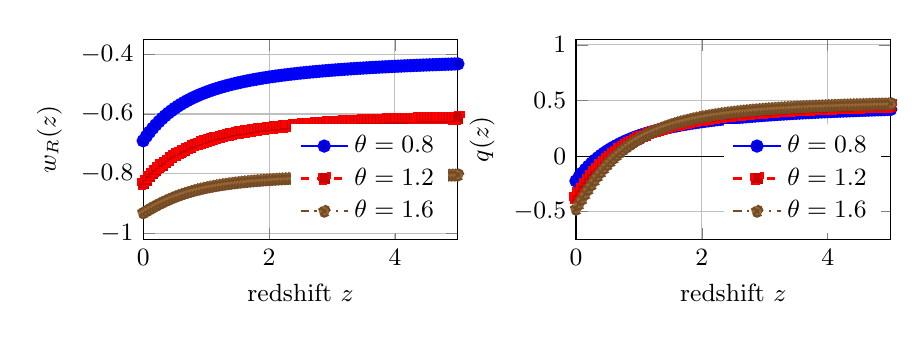
\begin{tikzpicture}
\begin{groupplot}[
  group style={group size=2 by 1, horizontal sep=1.5cm},
  width=0.46\textwidth,
  height=0.34\textwidth,
  grid=both,
  xmin=0, xmax=5,
  legend style={font=\small, draw=none},
  tick label style={font=\small},
  label style={font=\small}
]
\nextgroupplot[
  xlabel={redshift \(z\)},
  ylabel={\(w_R(z)\)},
  ymin=-1.02, ymax=-0.35,
  legend pos=south east
]
\addplot+[thick] coordinates {
(0.0000,-0.68955994)
(0.0500,-0.67463575)
(0.1000,-0.66081693)
(0.1500,-0.64802549)
(0.2000,-0.63618249)
(0.2500,-0.62521096)
(0.3000,-0.61503771)
(0.3500,-0.60559426)
(0.4000,-0.59681732)
(0.4500,-0.58864885)
(0.5000,-0.58103592)
(0.5500,-0.57393048)
(0.6000,-0.56728897)
(0.6500,-0.56107201)
(0.7000,-0.55524401)
(0.7500,-0.54977280)
(0.8000,-0.54462932)
(0.8500,-0.53978731)
(0.9000,-0.53522298)
(0.9500,-0.53091482)
(1.0000,-0.52684330)
(1.0500,-0.52299072)
(1.1000,-0.51934097)
(1.1500,-0.51587940)
(1.2000,-0.51259266)
(1.2500,-0.50946857)
(1.3000,-0.50649600)
(1.3500,-0.50366476)
(1.4000,-0.50096551)
(1.4500,-0.49838969)
(1.5000,-0.49592942)
(1.5500,-0.49357747)
(1.6000,-0.49132717)
(1.6500,-0.48917234)
(1.7000,-0.48710732)
(1.7500,-0.48512684)
(1.8000,-0.48322603)
(1.8500,-0.48140037)
(1.9000,-0.47964567)
(1.9500,-0.47795805)
(2.0000,-0.47633387)
(2.0500,-0.47476976)
(2.1000,-0.47326258)
(2.1500,-0.47180938)
(2.2000,-0.47040743)
(2.2500,-0.46905416)
(2.3000,-0.46774716)
(2.3500,-0.46648420)
(2.4000,-0.46526315)
(2.4500,-0.46408203)
(2.5000,-0.46293899)
(2.5500,-0.46183228)
(2.6000,-0.46076024)
(2.6500,-0.45972133)
(2.7000,-0.45871408)
(2.7500,-0.45773712)
(2.8000,-0.45678914)
(2.8500,-0.45586892)
(2.9000,-0.45497528)
(2.9500,-0.45410714)
(3.0000,-0.45326344)
(3.0500,-0.45244320)
(3.1000,-0.45164549)
(3.1500,-0.45086941)
(3.2000,-0.45011413)
(3.2500,-0.44937885)
(3.3000,-0.44866280)
(3.3500,-0.44796526)
(3.4000,-0.44728555)
(3.4500,-0.44662300)
(3.5000,-0.44597699)
(3.5500,-0.44534694)
(3.6000,-0.44473227)
(3.6500,-0.44413244)
(3.7000,-0.44354694)
(3.7500,-0.44297526)
(3.8000,-0.44241695)
(3.8500,-0.44187155)
(3.9000,-0.44133863)
(3.9500,-0.44081777)
(4.0000,-0.44030859)
(4.0500,-0.43981070)
(4.1000,-0.43932375)
(4.1500,-0.43884738)
(4.2000,-0.43838126)
(4.2500,-0.43792508)
(4.3000,-0.43747853)
(4.3500,-0.43704131)
(4.4000,-0.43661314)
(4.4500,-0.43619375)
(4.5000,-0.43578288)
(4.5500,-0.43538027)
(4.6000,-0.43498570)
(4.6500,-0.43459892)
(4.7000,-0.43421971)
(4.7500,-0.43384786)
(4.8000,-0.43348316)
(4.8500,-0.43312541)
(4.9000,-0.43277442)
(4.9500,-0.43243000)
(5.0000,-0.43209197)
};
\addlegendentry{\(\theta=0.8\)}
\addplot+[thick,dashed] coordinates {
(0.0000,-0.83327500)
(0.0500,-0.82139201)
(0.1000,-0.81007780)
(0.1500,-0.79935155)
(0.2000,-0.78921706)
(0.2500,-0.77966658)
(0.3000,-0.77068398)
(0.3500,-0.76224740)
(0.4000,-0.75433124)
(0.4500,-0.74690780)
(0.5000,-0.73994844)
(0.5500,-0.73342444)
(0.6000,-0.72730759)
(0.6500,-0.72157066)
(0.7000,-0.71618766)
(0.7500,-0.71113396)
(0.8000,-0.70638642)
(0.8500,-0.70192339)
(0.9000,-0.69772469)
(0.9500,-0.69377159)
(1.0000,-0.69004672)
(1.0500,-0.68653402)
(1.1000,-0.68321862)
(1.1500,-0.68008682)
(1.2000,-0.67712596)
(1.2500,-0.67432437)
(1.3000,-0.67167127)
(1.3500,-0.66915672)
(1.4000,-0.66677155)
(1.4500,-0.66450728)
(1.5000,-0.66235609)
(1.5500,-0.66031075)
(1.6000,-0.65836457)
(1.6500,-0.65651135)
(1.7000,-0.65474538)
(1.7500,-0.65306133)
(1.8000,-0.65145427)
(1.8500,-0.64991965)
(1.9000,-0.64845321)
(1.9500,-0.64705100)
(2.0000,-0.64570936)
(2.0500,-0.64442486)
(2.1000,-0.64319432)
(2.1500,-0.64201477)
(2.2000,-0.64088344)
(2.2500,-0.63979773)
(2.3000,-0.63875524)
(2.3500,-0.63775368)
(2.4000,-0.63679096)
(2.4500,-0.63586507)
(2.5000,-0.63497416)
(2.5500,-0.63411648)
(2.6000,-0.63329040)
(2.6500,-0.63249438)
(2.7000,-0.63172695)
(2.7500,-0.63098678)
(2.8000,-0.63027256)
(2.8500,-0.62958309)
(2.9000,-0.62891724)
(2.9500,-0.62827392)
(3.0000,-0.62765212)
(3.0500,-0.62705090)
(3.1000,-0.62646933)
(3.1500,-0.62590656)
(3.2000,-0.62536179)
(3.2500,-0.62483424)
(3.3000,-0.62432319)
(3.3500,-0.62382795)
(3.4000,-0.62334787)
(3.4500,-0.62288233)
(3.5000,-0.62243073)
(3.5500,-0.62199252)
(3.6000,-0.62156717)
(3.6500,-0.62115418)
(3.7000,-0.62075305)
(3.7500,-0.62036334)
(3.8000,-0.61998461)
(3.8500,-0.61961645)
(3.9000,-0.61925845)
(3.9500,-0.61891025)
(4.0000,-0.61857148)
(4.0500,-0.61824180)
(4.1000,-0.61792088)
(4.1500,-0.61760841)
(4.2000,-0.61730409)
(4.2500,-0.61700763)
(4.3000,-0.61671877)
(4.3500,-0.61643723)
(4.4000,-0.61616277)
(4.4500,-0.61589515)
(4.5000,-0.61563413)
(4.5500,-0.61537951)
(4.6000,-0.61513106)
(4.6500,-0.61488859)
(4.7000,-0.61465190)
(4.7500,-0.61442080)
(4.8000,-0.61419512)
(4.8500,-0.61397469)
(4.9000,-0.61375934)
(4.9500,-0.61354890)
(5.0000,-0.61334324)
};
\addlegendentry{\(\theta=1.2\)}
\addplot+[thick,dashdotted] coordinates {
(0.0000,-0.93020611)
(0.0500,-0.92391970)
(0.1000,-0.91777406)
(0.1500,-0.91180817)
(0.2000,-0.90605177)
(0.2500,-0.90052619)
(0.3000,-0.89524549)
(0.3500,-0.89021746)
(0.4000,-0.88544480)
(0.4500,-0.88092612)
(0.5000,-0.87665683)
(0.5500,-0.87262994)
(0.6000,-0.86883672)
(0.6500,-0.86526727)
(0.7000,-0.86191093)
(0.7500,-0.85875666)
(0.8000,-0.85579330)
(0.8500,-0.85300976)
(0.9000,-0.85039522)
(0.9500,-0.84793919)
(1.0000,-0.84563162)
(1.0500,-0.84346294)
(1.1000,-0.84142406)
(1.1500,-0.83950644)
(1.2000,-0.83770201)
(1.2500,-0.83600325)
(1.3000,-0.83440311)
(1.3500,-0.83289500)
(1.4000,-0.83147280)
(1.4500,-0.83013081)
(1.5000,-0.82886371)
(1.5500,-0.82766657)
(1.6000,-0.82653481)
(1.6500,-0.82546419)
(1.7000,-0.82445074)
(1.7500,-0.82349081)
(1.8000,-0.82258098)
(1.8500,-0.82171809)
(1.9000,-0.82089921)
(1.9500,-0.82012161)
(2.0000,-0.81938274)
(2.0500,-0.81868024)
(2.1000,-0.81801193)
(2.1500,-0.81737576)
(2.2000,-0.81676983)
(2.2500,-0.81619236)
(2.3000,-0.81564171)
(2.3500,-0.81511633)
(2.4000,-0.81461478)
(2.4500,-0.81413573)
(2.5000,-0.81367792)
(2.5500,-0.81324017)
(2.6000,-0.81282139)
(2.6500,-0.81242056)
(2.7000,-0.81203671)
(2.7500,-0.81166895)
(2.8000,-0.81131642)
(2.8500,-0.81097834)
(2.9000,-0.81065397)
(2.9500,-0.81034260)
(3.0000,-0.81004358)
(3.0500,-0.80975630)
(3.1000,-0.80948018)
(3.1500,-0.80921466)
(3.2000,-0.80895923)
(3.2500,-0.80871342)
(3.3000,-0.80847675)
(3.3500,-0.80824881)
(3.4000,-0.80802919)
(3.4500,-0.80781749)
(3.5000,-0.80761336)
(3.5500,-0.80741646)
(3.6000,-0.80722645)
(3.6500,-0.80704304)
(3.7000,-0.80686593)
(3.7500,-0.80669485)
(3.8000,-0.80652953)
(3.8500,-0.80636973)
(3.9000,-0.80621522)
(3.9500,-0.80606576)
(4.0000,-0.80592116)
(4.0500,-0.80578120)
(4.1000,-0.80564570)
(4.1500,-0.80551448)
(4.2000,-0.80538736)
(4.2500,-0.80526418)
(4.3000,-0.80514479)
(4.3500,-0.80502903)
(4.4000,-0.80491676)
(4.4500,-0.80480785)
(4.5000,-0.80470217)
(4.5500,-0.80459959)
(4.6000,-0.80450000)
(4.6500,-0.80440329)
(4.7000,-0.80430935)
(4.7500,-0.80421808)
(4.8000,-0.80412937)
(4.8500,-0.80404315)
(4.9000,-0.80395931)
(4.9500,-0.80387777)
(5.0000,-0.80379846)
};
\addlegendentry{\(\theta=1.6\)}

\nextgroupplot[
  xlabel={redshift \(z\)},
  ylabel={\(q(z)\)},
  ymin=-0.75, ymax=1.05,
  legend pos=south east
]
\addplot+[thick] coordinates {
(0.0000,-0.22389984)
(0.0500,-0.18658938)
(0.1000,-0.15204232)
(0.1500,-0.12006372)
(0.2000,-0.09045622)
(0.2500,-0.06302740)
(0.3000,-0.03759426)
(0.3500,-0.01398564)
(0.4000,0.00795671)
(0.4500,0.02837788)
(0.5000,0.04741019)
(0.5500,0.06517380)
(0.6000,0.08177758)
(0.6500,0.09731998)
(0.7000,0.11188999)
(0.7500,0.12556801)
(0.8000,0.13842670)
(0.8500,0.15053174)
(0.9000,0.16194255)
(0.9500,0.17271295)
(1.0000,0.18289174)
(1.0500,0.19252320)
(1.1000,0.20164758)
(1.1500,0.21030150)
(1.2000,0.21851835)
(1.2500,0.22632857)
(1.3000,0.23376000)
(1.3500,0.24083810)
(1.4000,0.24758623)
(1.4500,0.25402578)
(1.5000,0.26017644)
(1.5500,0.26605631)
(1.6000,0.27168208)
(1.6500,0.27706914)
(1.7000,0.28223170)
(1.7500,0.28718290)
(1.8000,0.29193494)
(1.8500,0.29649908)
(1.9000,0.30088581)
(1.9500,0.30510488)
(2.0000,0.30916533)
(2.0500,0.31307560)
(2.1000,0.31684356)
(2.1500,0.32047655)
(2.2000,0.32398142)
(2.2500,0.32736460)
(2.3000,0.33063209)
(2.3500,0.33378951)
(2.4000,0.33684213)
(2.4500,0.33979492)
(2.5000,0.34265252)
(2.5500,0.34541931)
(2.6000,0.34809940)
(2.6500,0.35069668)
(2.7000,0.35321479)
(2.7500,0.35565720)
(2.8000,0.35802714)
(2.8500,0.36032770)
(2.9000,0.36256179)
(2.9500,0.36473216)
(3.0000,0.36684140)
(3.0500,0.36889200)
(3.1000,0.37088628)
(3.1500,0.37282647)
(3.2000,0.37471466)
(3.2500,0.37655288)
(3.3000,0.37834300)
(3.3500,0.38008685)
(3.4000,0.38178614)
(3.4500,0.38344250)
(3.5000,0.38505751)
(3.5500,0.38663265)
(3.6000,0.38816932)
(3.6500,0.38966890)
(3.7000,0.39113266)
(3.7500,0.39256184)
(3.8000,0.39395762)
(3.8500,0.39532113)
(3.9000,0.39665343)
(3.9500,0.39795557)
(4.0000,0.39922853)
(4.0500,0.40047325)
(4.1000,0.40169063)
(4.1500,0.40288155)
(4.2000,0.40404684)
(4.2500,0.40518730)
(4.3000,0.40630368)
(4.3500,0.40739674)
(4.4000,0.40846716)
(4.4500,0.40951563)
(4.5000,0.41054281)
(4.5500,0.41154931)
(4.6000,0.41253575)
(4.6500,0.41350270)
(4.7000,0.41445072)
(4.7500,0.41538035)
(4.8000,0.41629210)
(4.8500,0.41718648)
(4.9000,0.41806396)
(4.9500,0.41892501)
(5.0000,0.41977008)
};
\addlegendentry{\(\theta=0.8\)}
\addplot+[thick,dashed] coordinates {
(0.0000,-0.37478126)
(0.0500,-0.33022004)
(0.1000,-0.28779176)
(0.1500,-0.24756832)
(0.2000,-0.20956399)
(0.2500,-0.17374968)
(0.3000,-0.14006494)
(0.3500,-0.10842774)
(0.4000,-0.07874214)
(0.4500,-0.05090426)
(0.5000,-0.02480667)
(0.5500,-0.00034163)
(0.6000,0.02259655)
(0.6500,0.04411001)
(0.7000,0.06429627)
(0.7500,0.08324764)
(0.8000,0.10105092)
(0.8500,0.11778729)
(0.9000,0.13353240)
(0.9500,0.14835653)
(1.0000,0.16232479)
(1.0500,0.17549744)
(1.1000,0.18793019)
(1.1500,0.19967443)
(1.2000,0.21077765)
(1.2500,0.22128362)
(1.3000,0.23123274)
(1.3500,0.24066230)
(1.4000,0.24960669)
(1.4500,0.25809770)
(1.5000,0.26616465)
(1.5500,0.27383468)
(1.6000,0.28113287)
(1.6500,0.28808242)
(1.7000,0.29470484)
(1.7500,0.30102003)
(1.8000,0.30704647)
(1.8500,0.31280131)
(1.9000,0.31830046)
(1.9500,0.32355874)
(2.0000,0.32858990)
(2.0500,0.33340677)
(2.1000,0.33802129)
(2.1500,0.34244460)
(2.2000,0.34668710)
(2.2500,0.35075850)
(2.3000,0.35466786)
(2.3500,0.35842369)
(2.4000,0.36203392)
(2.4500,0.36550600)
(2.5000,0.36884690)
(2.5500,0.37206318)
(2.6000,0.37516099)
(2.6500,0.37814609)
(2.7000,0.38102392)
(2.7500,0.38379959)
(2.8000,0.38647791)
(2.8500,0.38906341)
(2.9000,0.39156037)
(2.9500,0.39397281)
(3.0000,0.39630453)
(3.0500,0.39855914)
(3.1000,0.40074002)
(3.1500,0.40285040)
(3.2000,0.40489329)
(3.2500,0.40687160)
(3.3000,0.40878803)
(3.3500,0.41064518)
(3.4000,0.41244548)
(3.4500,0.41419128)
(3.5000,0.41588477)
(3.5500,0.41752805)
(3.6000,0.41912311)
(3.6500,0.42067184)
(3.7000,0.42217606)
(3.7500,0.42363747)
(3.8000,0.42505770)
(3.8500,0.42643832)
(3.9000,0.42778080)
(3.9500,0.42908656)
(4.0000,0.43035694)
(4.0500,0.43159325)
(4.1000,0.43279669)
(4.1500,0.43396845)
(4.2000,0.43510966)
(4.2500,0.43622137)
(4.3000,0.43730462)
(4.3500,0.43836039)
(4.4000,0.43938961)
(4.4500,0.44039320)
(4.5000,0.44137200)
(4.5500,0.44232684)
(4.6000,0.44325852)
(4.6500,0.44416779)
(4.7000,0.44505538)
(4.7500,0.44592199)
(4.8000,0.44676828)
(4.8500,0.44759491)
(4.9000,0.44840249)
(4.9500,0.44919161)
(5.0000,0.44996284)
};
\addlegendentry{\(\theta=1.2\)}
\addplot+[thick,dashdotted] coordinates {
(0.0000,-0.47654584)
(0.0500,-0.42939776)
(0.1000,-0.38330546)
(0.1500,-0.33856129)
(0.2000,-0.29538824)
(0.2500,-0.25394646)
(0.3000,-0.21434115)
(0.3500,-0.17663092)
(0.4000,-0.14083601)
(0.4500,-0.10694591)
(0.5000,-0.07492623)
(0.5500,-0.04472454)
(0.6000,-0.01627541)
(0.6500,0.01049547)
(0.7000,0.03566801)
(0.7500,0.05932503)
(0.8000,0.08155028)
(0.8500,0.10242681)
(0.9000,0.12203586)
(0.9500,0.14045607)
(1.0000,0.15776281)
(1.0500,0.17402795)
(1.1000,0.18931952)
(1.1500,0.20370173)
(1.2000,0.21723491)
(1.2500,0.22997561)
(1.3000,0.24197669)
(1.3500,0.25328749)
(1.4000,0.26395398)
(1.4500,0.27401895)
(1.5000,0.28352221)
(1.5500,0.29250074)
(1.6000,0.30098889)
(1.6500,0.30901858)
(1.7000,0.31661942)
(1.7500,0.32381893)
(1.8000,0.33064265)
(1.8500,0.33711429)
(1.9000,0.34325591)
(1.9500,0.34908796)
(2.0000,0.35462949)
(2.0500,0.35989818)
(2.1000,0.36491050)
(2.1500,0.36968178)
(2.2000,0.37422627)
(2.2500,0.37855727)
(2.3000,0.38268718)
(2.3500,0.38662754)
(2.4000,0.39038913)
(2.4500,0.39398203)
(2.5000,0.39741563)
(2.5500,0.40069873)
(2.6000,0.40383956)
(2.6500,0.40684580)
(2.7000,0.40972467)
(2.7500,0.41248291)
(2.8000,0.41512685)
(2.8500,0.41766244)
(2.9000,0.42009524)
(2.9500,0.42243049)
(3.0000,0.42467311)
(3.0500,0.42682773)
(3.1000,0.42889868)
(3.1500,0.43089007)
(3.2000,0.43280576)
(3.2500,0.43464938)
(3.3000,0.43642435)
(3.3500,0.43813391)
(3.4000,0.43978111)
(3.4500,0.44136883)
(3.5000,0.44289980)
(3.5500,0.44437658)
(3.6000,0.44580161)
(3.6500,0.44717720)
(3.7000,0.44850552)
(3.7500,0.44978864)
(3.8000,0.45102851)
(3.8500,0.45222700)
(3.9000,0.45338587)
(3.9500,0.45450677)
(4.0000,0.45559131)
(4.0500,0.45664098)
(4.1000,0.45765722)
(4.1500,0.45864139)
(4.2000,0.45959478)
(4.2500,0.46051862)
(4.3000,0.46141409)
(4.3500,0.46228230)
(4.4000,0.46312431)
(4.4500,0.46394114)
(4.5000,0.46473376)
(4.5500,0.46550309)
(4.6000,0.46624999)
(4.6500,0.46697533)
(4.7000,0.46767989)
(4.7500,0.46836444)
(4.8000,0.46902971)
(4.8500,0.46967640)
(4.9000,0.47030519)
(4.9500,0.47091670)
(5.0000,0.47151156)
};
\addlegendentry{\(\theta=1.6\)}
\addplot[black,thin,mark=none] coordinates {(0,0) (5,0)};
\end{groupplot}
\end{tikzpicture}
\caption{Cosmological dynamics evaluated from the homogeneous RFG equations and rendered from numerical coordinates embedded in this \LaTeX{} source. The left panel shows \(w_R(z)\), and the right panel shows \(q(z)\), for three representative values of \(\theta\). The acceleration transition \(q=0\) coincides with \(\Omega_R(z_{\rm acc})=1/(1+\theta)\). Parameters: \(\Omega_{m0}=0.3\), \(\Omega_{r0}=9\times10^{-5}\), and \(\Omega_{R0}=1-\Omega_{m0}-\Omega_{r0}\).}
\label{fig:cosmo}
\end{figure}
\FloatBarrier

\subsection{Early- and late-time asymptotics}

At early times \(E\to\infty\), so \(\Omega_R=\Omega_{R0}E^{-\theta}\to0\). The standard radiation- and matter-dominated limits are therefore recovered. The future attractor is de~Sitter with
\[
E_\infty=\Omega_{R0}^{1/\theta},\qquad H_\infty=H_0\Omega_{R0}^{1/\theta}.
\]

\subsection{Tensor sector and standard-siren ratio}

The quadratic action for transverse-traceless modes is
\begin{equation}
S_T^{(2)}=\frac{\mpl^2}{8}\int\dd t\,\dd^3x\,a^3Q_T\Bigl[\dot h_{ij}\dot h_{ij}-\frac{\partial_k h_{ij}\partial_k h_{ij}}{a^2}\Bigr],
\end{equation}
with
\[
\Boxed{Q_T(a)=1-\frac{\Omega_R(a)}{1+\theta},\qquad c_T^2=1.}
\]
The no-ghost condition \(Q_T>0\) holds throughout the homogeneous branch for \(\theta>0\). The standard-siren amplitude relation follows at once:
\begin{equation}
\Boxed{\frac{d_L^{\rm GW}(z)}{d_L^{\rm EM}(z)}=\sqrt{\frac{Q_T(0)}{Q_T(z)}}.}
\label{eq:siren}
\end{equation}

Equation~\eqref{eq:siren} is the WKB/subhorizon tensor-amplitude result under the following assumptions: matter is minimally coupled to the metric \(g_{\mu\nu}\), photons and gravitational waves share the same background redshift relation, there is no tensor mixing with an additional propagating spin--2 field, and the observed Planck normalization is fixed at \(z=0\). Under these assumptions \(Q_T\) modifies only the tensor friction term, not the null cone, which is why \(c_T=1\) and the distance ratio in Eq.~\eqref{eq:siren} can differ from unity simultaneously.

\begin{remark}[Order-of-magnitude estimate]
For a representative late-time branch with \(\Omega_{R0}\approx0.7\) and \(\theta\approx1.6\) one obtains \(Q_T(0)\approx0.73\). At high redshift \(\Omega_R\to0\), so \(Q_T\to1\) and the ratio approaches \(\sqrt{Q_T(0)}\approx0.85\). At redshift \(z=1\) the same branch yields a ratio of order \(0.9\). The near-luminal propagation constraint from GW170817 is automatically respected because \(c_T=1\)~\cite{GW170817}. The amplitude-distance modification is instead a standard-siren observable of the type discussed in forecast studies~\cite{Belgacem}. The corresponding curve is shown in Fig.~\ref{fig:siren}. A dedicated likelihood comparison is left for future work.
\end{remark}

\begin{figure}[H]
\centering
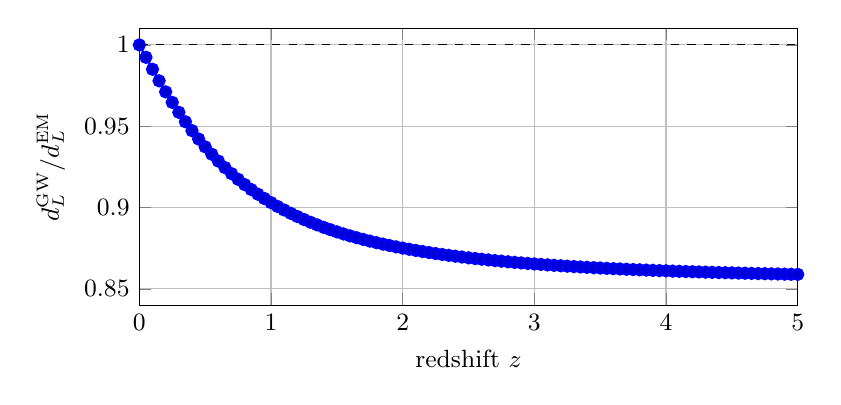
\begin{tikzpicture}
\begin{axis}[
  width=0.82\textwidth,
  height=0.42\textwidth,
  xlabel={redshift \(z\)},
  ylabel={\(d_L^{\rm GW}/d_L^{\rm EM}\)},
  xmin=0, xmax=5,
  ymin=0.84, ymax=1.01,
  grid=both,
  tick label style={font=\small},
  label style={font=\small}
]
\addplot+[thick] coordinates {
(0.0000,1.00000000)
(0.0500,0.99238993)
(0.1000,0.98501840)
(0.1500,0.97792548)
(0.2000,0.97113918)
(0.2500,0.96467707)
(0.3000,0.95854805)
(0.3500,0.95275393)
(0.4000,0.94729098)
(0.4500,0.94215130)
(0.5000,0.93732390)
(0.5500,0.93279569)
(0.6000,0.92855222)
(0.6500,0.92457829)
(0.7000,0.92085841)
(0.7500,0.91737715)
(0.8000,0.91411937)
(0.8500,0.91107048)
(0.9000,0.90821647)
(0.9500,0.90554405)
(1.0000,0.90304066)
(1.0500,0.90069451)
(1.1000,0.89849456)
(1.1500,0.89643050)
(1.2000,0.89449276)
(1.2500,0.89267243)
(1.3000,0.89096124)
(1.3500,0.88935156)
(1.4000,0.88783631)
(1.4500,0.88640892)
(1.5000,0.88506335)
(1.5500,0.88379399)
(1.6000,0.88259568)
(1.6500,0.88146362)
(1.7000,0.88039340)
(1.7500,0.87938091)
(1.8000,0.87842238)
(1.8500,0.87751431)
(1.9000,0.87665344)
(1.9500,0.87583678)
(2.0000,0.87506154)
(2.0500,0.87432514)
(2.1000,0.87362518)
(2.1500,0.87295943)
(2.2000,0.87232583)
(2.2500,0.87172246)
(2.3000,0.87114753)
(2.3500,0.87059937)
(2.4000,0.87007644)
(2.4500,0.86957729)
(2.5000,0.86910057)
(2.5500,0.86864503)
(2.6000,0.86820949)
(2.6500,0.86779285)
(2.7000,0.86739408)
(2.7500,0.86701224)
(2.8000,0.86664641)
(2.8500,0.86629575)
(2.9000,0.86595948)
(2.9500,0.86563685)
(3.0000,0.86532717)
(3.0500,0.86502978)
(3.1000,0.86474407)
(3.1500,0.86446946)
(3.2000,0.86420540)
(3.2500,0.86395140)
(3.3000,0.86370695)
(3.3500,0.86347162)
(3.4000,0.86324496)
(3.4500,0.86302658)
(3.5000,0.86281609)
(3.5500,0.86261314)
(3.6000,0.86241737)
(3.6500,0.86222848)
(3.7000,0.86204614)
(3.7500,0.86187009)
(3.8000,0.86170003)
(3.8500,0.86153571)
(3.9000,0.86137689)
(3.9500,0.86122333)
(4.0000,0.86107482)
(4.0500,0.86093113)
(4.1000,0.86079207)
(4.1500,0.86065746)
(4.2000,0.86052711)
(4.2500,0.86040084)
(4.3000,0.86027850)
(4.3500,0.86015994)
(4.4000,0.86004500)
(4.4500,0.85993354)
(4.5000,0.85982542)
(4.5500,0.85972053)
(4.6000,0.85961874)
(4.6500,0.85951992)
(4.7000,0.85942398)
(4.7500,0.85933080)
(4.8000,0.85924028)
(4.8500,0.85915233)
(4.9000,0.85906685)
(4.9500,0.85898375)
(5.0000,0.85890295)
};
\addplot[black,thin,dashed,mark=none] coordinates {(0,1) (5,1)};
\end{axis}
\end{tikzpicture}
\caption{Standard-siren prediction evaluated from Eq.~\eqref{eq:siren} on the homogeneous RFG background and rendered from numerical coordinates embedded in this \LaTeX{} source, for \(\Omega_{R0}=0.70\) and \(\theta=1.6\). The ratio equals unity at \(z=0\), is approximately \(0.903\) at \(z=1\), and approaches \(\sqrt{Q_T(0)}\approx0.855\) at high redshift. No illustrative observational point is added, because a statistically meaningful comparison requires an explicit likelihood analysis.}
\label{fig:siren}
\end{figure}
\FloatBarrier


%====================================================
\section{RFG-R: regular multiscale effective completion}
\label{sec:rfg-r}

The original branch in Eqs.~\eqref{eq:Q}--\eqref{eq:V} is singular at
\(X=0\) when \(\theta>0\). It therefore cannot by itself support a standard
asymptotically flat weak-field expansion. This section defines a different,
low-energy effective theory, called RFG-R. It is constructed to retain the
cosmological branch to a controlled accuracy, to be regular at \(X=0\), and
to state the local matching rule rather than silently extrapolating a
homogeneous action into Solar-System geometry. RFG-R is a model definition;
it is not claimed to follow uniquely from the original RFG action.

\subsection{Regular cosmological action and exact reconstruction}

Let \(p\) be an even integer satisfying \(p>\theta\), let
\(\epsilon>0\), and define
\begin{equation}
 \nu:=1+\frac{\theta}{p},\qquad
 A:=\frac{\Omega_{R0}}{1+\theta}.
\end{equation}
The regular response and tensor normalization are
\begin{align}
 \mathcal R_\epsilon(X)&:=
 \Omega_{R0}\frac{X^{p+2}}{\left(X^p+\epsilon^p\right)^\nu},
 \label{eq:RFGR-response}\\
 Q_\epsilon(X)&:=1-A\frac{X^p}{\left(X^p+\epsilon^p\right)^\nu}.
 \label{eq:RFGR-Q}
\end{align}
The cosmological RFG-R action is
\begin{equation}
 S_{\rm cos}=\frac{\mpl^2}{2}\int\dd^4x\sqrt{-g}\,
 \left[Q_\epsilon(X)\left({}^{(3)}R+K_{\mu\nu}K^{\mu\nu}-K^2\right)
 +2H_0^2V_\epsilon(X)\right]+S_m[g,\Psi].
 \label{eq:RFGR-cosmological-action}
\end{equation}
Matter is minimally and universally coupled to the Jordan metric \(g_{\mu\nu}\).
Define
\begin{equation}
 F_\epsilon(X):=X^2-\mathcal R_\epsilon(X)-X^2Q_\epsilon(X)
 -X^3Q_{\epsilon,X}(X).
 \label{eq:RFGR-F}
\end{equation}
The FLRW lapse equation has the target form
\begin{equation}
 \boxed{E^2=\Omega_{m0}a^{-3}+\Omega_{r0}a^{-4}+\mathcal R_\epsilon(E).}
 \label{eq:RFGR-background}
\end{equation}
Comparison with Eq.~\eqref{eq:FLRW-constraint-general} fixes the potential,
up to the usual ADM boundary representative \(CX\), through
\begin{align}
 V_\epsilon-XV_{\epsilon,X}&=3F_\epsilon(X),\\
 \boxed{V_\epsilon(X)=-3X\int_0^X\frac{F_\epsilon(s)}{s^2}\,\dd s.}
 \label{eq:RFGR-potential}
\end{align}
The integrand is finite at the origin. Thus Eq.~\eqref{eq:RFGR-potential} is
an action-level reconstruction, not a background-only prescription.

For \(X\gg\epsilon\),
\begin{align}
 \mathcal R_\epsilon(X)&=\Omega_{R0}X^{2-\theta}
 \left[1-\left(1+\frac{\theta}{p}\right)
 \left(\frac{\epsilon}{X}\right)^p+O\left((\epsilon/X)^{2p}\right)\right],\\
 Q_\epsilon(X)&=1-AX^{-\theta}
 \left[1-\left(1+\frac{\theta}{p}\right)
 \left(\frac{\epsilon}{X}\right)^p+O\left((\epsilon/X)^{2p}\right)\right].
 \label{eq:RFGR-recovery}
\end{align}
The reference choice \(p=4\), \(\epsilon=10^{-8}\), and \(\theta=1.6\)
therefore changes the original branch by at most \(2.5\times10^{-32}\) for
\(X\geq0.8\), analytically. At small \(X\), \(Q_\epsilon(0)=1\) and
\(V_\epsilon=O(X^{p+2})\), so the Einstein--Hilbert ADM kinetic operator is
recovered at \(K=0\).

\begin{figure}[H]
\centering
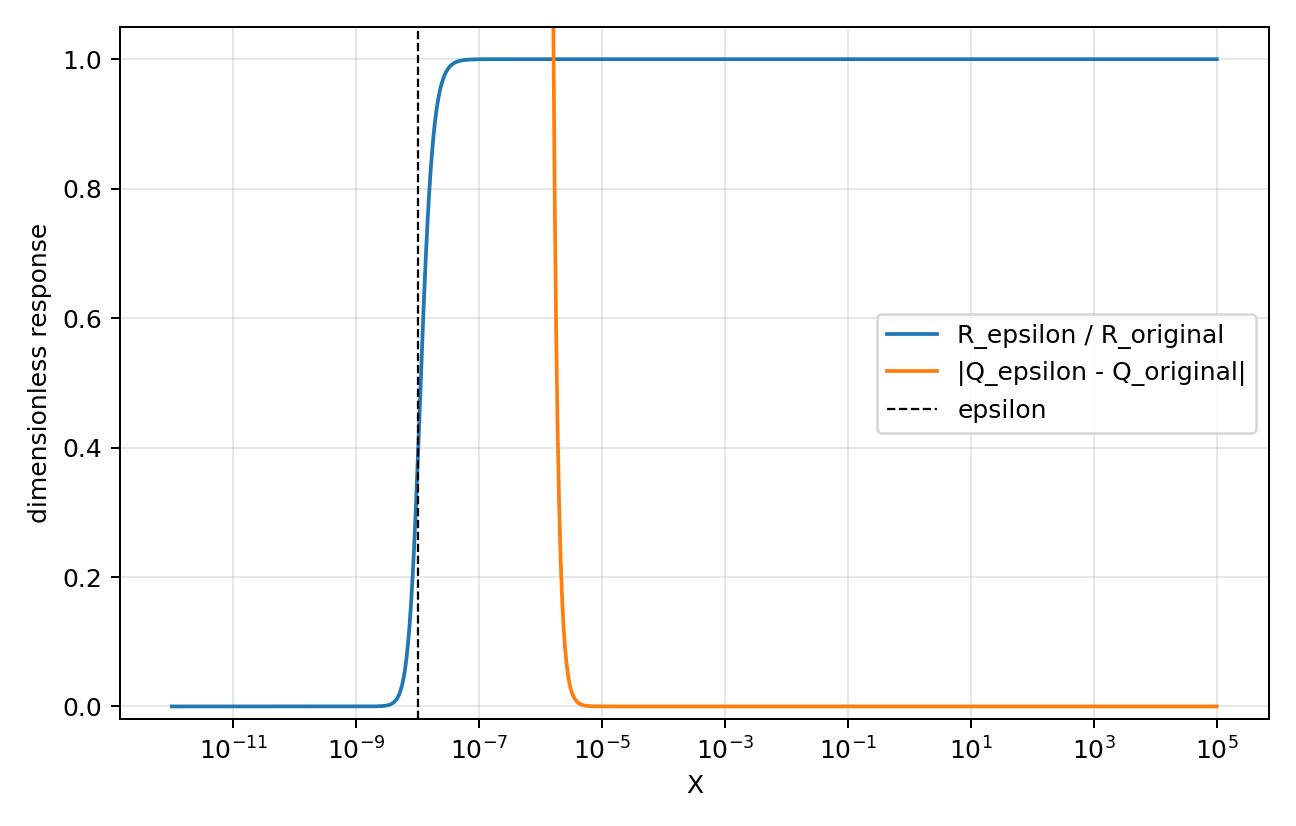
\includegraphics[width=0.82\textwidth]{r_universe_completion/generated/figures/regularization_recovery.png}
\caption{Numerical verification of the controlled high-\(X\) recovery of the
original RFG response by RFG-R. The source is
\RFGLocalPath{scripts/validate\_completion.py}; the generated data and all
parameters are included with this manuscript.}
\label{fig:RFGR-recovery}
\end{figure}

\subsection{Local GR matching and PPN statement}

The cosmological action is supplemented by an explicit multiscale matching
rule. Let
\begin{equation}
 W:=\frac{\sqrt{\lvert C_{\alpha\beta\gamma\delta}
 C^{\alpha\beta\gamma\delta}\rvert}}{(H_0/c)^2}.
 \label{eq:RFGR-Weyl}
\end{equation}
Choose a \(C^\infty\) switch \(s(W)\) with \(s=1\) for \(W\leq10^8\)
and \(s=0\) for \(W\geq10^9\); its explicit bump-function construction is
given in \RFGLocalPath{docs/completion\_derivation.md}. The complete
low-energy EFT is
\begin{equation}
 S_{\rm eff}=S_{\rm GR}+\int\dd^4x\,s(W)
 \left(\mathscr L_{\rm cos}-\mathscr L_{\rm GR}\right).
 \label{eq:RFGR-matching}
\end{equation}
Here \(\mathscr L\) denotes the corresponding covariant action density,
including \(\sqrt{-g}\). Flat FLRW has \(W=0\), hence uses the cosmological
action. In every open region with \(W\geq10^9\), both \(s\) and all its
derivatives vanish, so the action and all its variations are exactly those of
GR with the same universally coupled matter sector. For a Schwarzschild Sun,
\begin{equation}
 W(r)=\frac{\sqrt{48}\,GM_\odot/c^2}{r^3(H_0/c)^2},
 \qquad W(1\,{\rm AU})=5.756\times10^{22}
\end{equation}
at the stated reference point. The model prediction in that local domain is
therefore
\begin{equation}
 \boxed{\gamma_{\rm PPN}=\beta_{\rm PPN}=1,\qquad
 \alpha_1=\alpha_2=0.}
 \label{eq:RFGR-PPN}
\end{equation}
This is an EFT matching prediction, not a derivation of a microscopic
screening mechanism. The packaged Cassini Gaussian factor gives
\(-2\ln\mathcal L_{\rm Cassini}=0.833648\) for Eq.~\eqref{eq:RFGR-PPN}
and the reported measurement~\cite{Cassini}.

\subsection{Tensor and matter/CMB likelihood interface}

On FLRW, the tensor result is obtained from the same quadratic reduction as
before with \(Q\) replaced by \(Q_\epsilon\):
\begin{equation}
 Q_T(a)=Q_\epsilon(E(a))>0,\qquad c_T^2=1,\qquad
 \frac{d_L^{\rm GW}}{d_L^{\rm EM}}=
 \sqrt{\frac{Q_T(0)}{Q_T(z)}}.
 \label{eq:RFGR-siren}
\end{equation}
The reference validation grid has \(\min Q_T=0.6153848\).

The matter and CMB test is defined from the action derivatives, not from an
assumed quasi-static \(\mu(a,k)\). In particular,
\begin{align}
 \mathcal L_{{}^{(3)}R}&=Q_\epsilon,\\
 \mathcal L_{K_{ij}{}^{(3)}R}&=\frac{Q_{\epsilon,X}}{3H_0}\gamma^{ij},\\
 \mathcal L_{K_{ij}}&=2Q_\epsilon(K^{ij}-K\gamma^{ij})
 +\left[\frac{Q_{\epsilon,X}}{3H_0}
 \left({}^{(3)}R+K_{mn}K^{mn}-K^2\right)
 +\frac{2H_0}{3}V_{\epsilon,X}\right]\gamma^{ij}.
 \label{eq:RFGR-ADM-derivatives}
\end{align}
The full kinetic Hessian is obtained by differentiating
Eq.~\eqref{eq:RFGR-ADM-derivatives}. For every sampled cosmology, a full
3+1 Einstein--Boltzmann implementation must reject absent background roots,
\(Q_T\leq0\), ghosts, gradient instabilities, and singular constraint
matrices before computing
\(C_\ell^{TT,TE,EE}\), \(C_L^{\phi\phi}\), \(P(k,z)\),
\(f\sigma_8(z)\), and Eq.~\eqref{eq:RFGR-siren}. The intended joint
likelihood is
\begin{equation}
 \ln\mathcal L=\ln\mathcal L_{\rm Planck18}
 +\ln\mathcal L_{\rm lensing}+\ln\mathcal L_{\rm BAO}
 +\ln\mathcal L_{\rm SN}+\ln\mathcal L_{\rm RSD}
 +\ln\mathcal L_{\rm PPN}+\ln\mathcal L_{\rm GW}.
 \label{eq:RFGR-likelihood}
\end{equation}
The public calculation protocol, exact input/output contract, and deterministic
rejection conditions are supplied in
\RFGLocalPath{docs/likelihood\_pipeline.md}. The protocol is compatible with
the full 3+1 EFT route in H-EFTCAMB~\cite{EFTCAMB,HEFTCAMB} and with the
official Planck likelihoods~\cite{PlanckLikelihood}. It is intentionally not
a claim that the likelihood in Eq.~\eqref{eq:RFGR-likelihood} has already been
evaluated.

\subsection{Reproducibility and public links}

The self-contained supplement distributed beside this \LaTeX{} source is
\RFGLocalPath{README.md}. Its calculation manifest is
\RFGLocalPath{CALCULATION\_MANIFEST.md}; the executable validation command is
\texttt{bash r\_universe\_completion/scripts/run\_all.sh}. The permanent
public counterparts are linked directly from the paper:
\RFGRepoPath{docs/completion\_derivation.md},
\RFGRepoPath{docs/likelihood\_pipeline.md}, and
\RFGRepoPath{scripts/validate\_completion.py}. The repository directory also
contains the exact source of the manuscript, generated tables, figures, and
the standalone RFG-R completion article.

\section{Quadratic scalar geometry and constraint kernel}
\label{sec:quadratic_scalar}

This section develops the scalar perturbation sector directly from the RFG
action.  No auxiliary scalar field and no scalar--tensor closure assumption is introduced.
The only inputs are the preferred-foliation ADM variables and the functions
\(Q(X)\) and \(V(X)\) already fixed by the homogeneous reconstruction.

We use
\begin{equation}
N=1+\alpha,\qquad
N_i=\partial_i\beta,\qquad
\gamma_{ij}=a^2 e^{2\zeta}\delta_{ij},
\label{eq:scalar_adm_param}
\end{equation}
and
\begin{equation}
K_{ij}=\frac{1}{2N}
\left(\dot\gamma_{ij}-D_iN_j-D_jN_i\right),
\qquad
X=\frac{K}{3H_0}.
\label{eq:scalar_K_definition}
\end{equation}
All perturbative orders below refer to powers of
\(\alpha,\beta,\zeta\).

\subsection{Exact measure and intrinsic curvature}

\begin{lemma}[Measure expansion]
For the parametrization \eqref{eq:scalar_adm_param},
\begin{equation}
\sqrt{\gamma}=a^3e^{3\zeta},
\end{equation}
and hence
\begin{equation}
N\sqrt{\gamma}
=
a^3\left[
1+\alpha+3\zeta+3\alpha\zeta+\frac{9}{2}\zeta^2
\right]+O(3).
\label{eq:measure_second_order}
\end{equation}
\end{lemma}

\begin{proof}
The determinant is
\(\det\gamma_{ij}=a^6e^{6\zeta}\).  Taking its positive square root and
expanding the exponential gives \eqref{eq:measure_second_order}.  Because
\(N=1+\alpha\) is used as the perturbation variable, no independent
\(\alpha^2\) term occurs in the measure.
\end{proof}

\begin{lemma}[Intrinsic curvature expansion]
For \(\gamma_{ij}=a^2e^{2\zeta}\delta_{ij}\),
\begin{equation}
{}^{(3)}R
=
\frac{e^{-2\zeta}}{a^2}
\left[-4\partial^2\zeta-2(\partial\zeta)^2\right].
\label{eq:exact_3curvature}
\end{equation}
Consequently,
\begin{align}
R^{(1)}&=-\frac{4}{a^2}\partial^2\zeta,
\\
R^{(2)}&=
\frac{1}{a^2}
\left[
8\zeta\,\partial^2\zeta-2(\partial\zeta)^2
\right].
\label{eq:3curvature_orders}
\end{align}
\end{lemma}

\subsection{Extrinsic curvature and the relational perturbation}

Define
\begin{equation}
b\equiv\frac{\partial^2\beta}{a^2}.
\end{equation}
Direct contraction of \eqref{eq:scalar_K_definition} gives the exact trace
\begin{equation}
K=
\frac{1}{1+\alpha}
\left[
3(H+\dot\zeta)
-\frac{e^{-2\zeta}}{a^2}
\left(\partial^2\beta+\partial_i\zeta\,\partial_i\beta\right)
\right].
\label{eq:exact_K_scalar}
\end{equation}
Writing
\begin{equation}
K=3H+\delta K_1+\delta K_2+O(3),
\end{equation}
one obtains
\begin{align}
\delta K_1
&=
3\dot\zeta-3H\alpha-b,
\label{eq:deltaK1}
\\
\delta K_2
&=
3H\alpha^2-3\alpha\dot\zeta+\alpha b
-\frac{1}{a^2}\partial_i\zeta\,\partial_i\beta
+\frac{2\zeta}{a^2}\partial^2\beta.
\label{eq:deltaK2}
\end{align}
For a Fourier mode, let
\begin{equation}
u\equiv\dot\zeta-H\alpha,
\qquad
y\equiv\frac{k^2}{a^2}\beta.
\label{eq:u_y_def}
\end{equation}
Since \(b=-y\), the linear relational perturbation becomes
\begin{equation}
\boxed{\delta K_1=3u+y},
\qquad
\delta X_1=\frac{3u+y}{3H_0}.
\label{eq:deltaK1_uy}
\end{equation}

\subsection{Trace--shear decomposition}

Introduce the shear
\begin{equation}
\sigma_{ij}=K_{ij}-\frac{1}{3}K\gamma_{ij}.
\end{equation}
The exact algebraic identity
\begin{equation}
K_{ij}K^{ij}-K^2
=
\sigma_{ij}\sigma^{ij}-\frac{2}{3}K^2
\label{eq:trace_shear_identity}
\end{equation}
separates the trace response from the shift shear.  Since the background shear
vanishes, only its linear part is required at quadratic order:
\begin{equation}
\sigma_{ij}\sigma^{ij}
=
\frac{1}{a^4}
\left[
(\partial_i\partial_j\beta)^2
-\frac{1}{3}(\partial^2\beta)^2
\right]+O(3).
\label{eq:shear_square_position}
\end{equation}
For one Fourier mode this reduces to
\begin{equation}
\boxed{
\sigma_{ij}\sigma^{ij}=\frac{2}{3}y^2
}.
\label{eq:shear_square_fourier}
\end{equation}

\subsection{Equivalent scalar kernel of the RFG action}

Define
\begin{equation}
F(X)\equiv -3X^2Q(X)+V(X).
\label{eq:F_definition}
\end{equation}
Using \(K=3H_0X\) and \eqref{eq:trace_shear_identity}, the gravitational
action is identically rewritten as
\begin{equation}
S_g=
\frac{M_{\rm Pl}^2}{2}
\int dt\,d^3x\,N\sqrt{\gamma}
\left[
Q(X)\,{}^{(3)}R
+Q(X)\sigma_{ij}\sigma^{ij}
+2H_0^2F(X)
\right].
\label{eq:RFG_trace_shear_action}
\end{equation}
Equation \eqref{eq:RFG_trace_shear_action} is not an additional assumption; it is an
algebraically equivalent form of the original RFG action.

Let
\begin{equation}
\bar X=\frac{H}{H_0},
\qquad
\delta X_1=\frac{\delta K_1}{3H_0},
\qquad
\delta X_2=\frac{\delta K_2}{3H_0},
\end{equation}
and evaluate \(Q,F\) and their derivatives at \(\bar X\).  Before use of the
background equations or integrations by parts, the quadratic gravitational
density is
\begin{align}
\frac{\mathcal L_g^{(2)}}{(M_{\rm Pl}^2/2)a^3}
={}&
Q R^{(2)}
+\left[Q(\alpha+3\zeta)+Q_{,X}\delta X_1\right]R^{(1)}
+Q\,\sigma_{ij}\sigma^{ij}
\nonumber\\
&+2H_0^2
\Bigg[
F\left(3\alpha\zeta+\frac{9}{2}\zeta^2\right)
+F_{,X}
\left(
\delta X_2+(\alpha+3\zeta)\delta X_1
\right)
+\frac{1}{2}F_{,XX}\delta X_1^2
\Bigg].
\label{eq:quadratic_gravity_density_compact}
\end{align}

\begin{proposition}[RFG Hessian identity]
For
\begin{equation}
Q(X)=1-\frac{\Omega_{R0}}{1+\theta}X^{-\theta},
\end{equation}
and the reconstructed potential of the homogeneous RFG branch,
\begin{equation}
F(X)
=
-3X^2+\frac{3\Omega_{R0}}{1-\theta}X^{2-\theta},
\qquad
(\theta\neq1),
\label{eq:F_RFG}
\end{equation}
one has
\begin{equation}
F_{,XX}=-3D,
\qquad
D\equiv2-(2-\theta)\Omega_R,
\qquad
\Omega_R\equiv\Omega_{R0}X^{-\theta}.
\label{eq:Fxx_identity}
\end{equation}
\end{proposition}

\begin{proof}
Twice differentiating \eqref{eq:F_RFG} gives
\[
F_{,XX}
=
-6+3(2-\theta)\Omega_{R0}X^{-\theta}
=
-3\left[2-(2-\theta)\Omega_R\right].
\]
\end{proof}

The trace-Hessian contribution to the Fourier-space quadratic kernel therefore
takes the exact form
\begin{equation}
2H_0^2\left(\frac{1}{2}F_{,XX}\delta X_1^2\right)
=
-\frac{D}{3}(3u+y)^2,
\label{eq:trace_hessian_kernel}
\end{equation}
whereas the shear contribution is
\begin{equation}
Q\,\sigma_{ij}\sigma^{ij}
=
\frac{2Q}{3}y^2.
\label{eq:shear_kernel}
\end{equation}
Thus the lapse--shift kernel contains
\begin{equation}
\boxed{
-\frac{D}{3}(3u+y)^2+\frac{2Q}{3}y^2
}
\label{eq:lapse_shift_kernel}
\end{equation}
together with the curvature couplings displayed explicitly in
\eqref{eq:quadratic_gravity_density_compact}.

\subsection{Regular branch and the case \texorpdfstring{\(\theta=1\)}{theta=1}}

On the physical branch
\begin{equation}
0\leq\Omega_R<1,\qquad \theta>0,
\end{equation}
the coefficients obey
\begin{equation}
D=2(1-\Omega_R)+\theta\Omega_R>0,
\qquad
Q=1-\frac{\Omega_R}{1+\theta}>
\frac{\theta}{1+\theta}>0.
\label{eq:D_Q_positive}
\end{equation}
The trace and shear Hessians are therefore nondegenerate on this branch.

At \(\theta=1\), the regular logarithmic representative of the reconstructed
potential yields, up to an irrelevant linear term,
\begin{equation}
F_{\theta=1}(X)
=
-3X^2+3\Omega_{R0}X\ln X.
\end{equation}
Its second derivative is
\begin{equation}
F_{,XX}
=
-6+\frac{3\Omega_{R0}}{X}
=
-3(2-\Omega_R).
\end{equation}
Hence \eqref{eq:Fxx_identity} continues smoothly to
\begin{equation}
D=2-\Omega_R,
\end{equation}
and \(\theta=1\) is not a degeneracy of the quadratic scalar kernel.

\begin{remark}[Status of the scalar degree-of-freedom count]
Equations \eqref{eq:quadratic_gravity_density_compact}--\eqref{eq:lapse_shift_kernel}
give the unreduced quadratic gravitational action. The pure-gravity FLRW lapse--shift
reduction is now performed explicitly below. That calculation establishes that the
pure-gravity scalar principal sector has no independent propagating \(\dot\zeta^2\)
term. It does not by itself determine the nonperturbative Dirac rank of the full
metric--khronon theory, nor the matter-coupled scalar eigenvalues.
\end{remark}



\section{Verified scalar constraint identities}

The following identities have been verified directly from the quadratic expansion and are therefore recorded independently of the unresolved Hamiltonian reduction.

\begin{lemma}[Second derivative identity]
Defining
\[
D\equiv 2-(2-\theta)\Omega_R,
\]
the Hessian of the effective potential satisfies
\[
F_{XX}=-3D.
\]
\end{lemma}

\begin{proposition}[Quadratic trace--shear kernel]
Introducing
\[
u=\dot\zeta-H\alpha,
\qquad
y=\frac{k^2}{a^2}\beta,
\]
the quadratic kinetic kernel decomposes as
\[
-\frac{D}{3}(3u+y)^2+\frac23Q\,y^2.
\]
Hence the trace and shear sectors separate explicitly.
\end{proposition}

\begin{lemma}[$F_X$ block]
Using the explicit second-order expansion of $K$ and discarding only spatial boundary terms,
\[
\delta X_2+(\alpha+3\zeta)\delta X_1
\;\widehat{=}\;
\frac{3}{H_0}\zeta\,u.
\]
Consequently the $F_X$ contribution carries no independent dependence on the shift variable and therefore does not contribute to the momentum constraint after spatial integration by parts.
\end{lemma}

\begin{remark}
The identities above are the checks used in the exact reduction below. They are not
separate assumptions.
\end{remark}

\section{Exact pure-gravity FLRW scalar reduction}
\label{sec:exact_scalar_reduction}

This section incorporates the complete algebraic reduction of the pure-gravity scalar
kernel. It is the calculation that decides whether the FLRW quadratic scalar sector
contains an ordinary propagating gravitational scalar before matter is added.

Define
\begin{equation}
p\equiv\frac{k^2}{a^2},\qquad
N=1+\alpha,\qquad
N_i=\partial_i\beta,\qquad
y\equiv p\beta,
\qquad
u\equiv\dot\zeta-H\alpha .
\label{eq:scalar_reduction_variables}
\end{equation}
The scaled quadratic density is
\begin{equation}
L\equiv
\frac{\mathcal L_g^{(2)}}{(\mpl^2/2)a^3}.
\end{equation}
Keeping all terms contained in Eq.~\eqref{eq:quadratic_gravity_density_compact},
the scalar density is
\begin{align}
L={}&
-3DH^2\alpha^2+2DH\alpha y+6DH\alpha\dot\zeta
-\frac{D}{3}y^2-2Dy\dot\zeta-3D\dot\zeta^2
\nonumber\\
&+6FH_0^2\alpha\zeta
-6F_XHH_0\alpha\zeta
+6F_XH_0\zeta\dot\zeta
\nonumber\\
&-\frac{4HQ_X}{H_0}\alpha p\zeta
+4Q\alpha p\zeta
+\frac{2Q}{3}y^2
+\frac{4Q_X}{3H_0}py\zeta
+\frac{4Q_X}{H_0}p\zeta\dot\zeta .
\label{eq:scalar_full_L}
\end{align}
Here \(D,Q,Q_X,F,F_X,H\) are functions of the homogeneous background and are
held fixed during the algebraic lapse--shift elimination.

\subsection{Lapse and shift constraints}

Variation of Eq.~\eqref{eq:scalar_full_L} with respect to \(\alpha\) gives
\begin{equation}
\Boxed{
0=
-3DH^2\alpha+DHy+3DH\dot\zeta
+3FH_0^2\zeta-3F_XHH_0\zeta
-\frac{2HQ_X}{H_0}p\zeta
+2Qp\zeta .
}
\label{eq:alpha_constraint_exact}
\end{equation}
Variation with respect to \(y\) gives
\begin{equation}
\Boxed{
0=
-3DH\alpha+Dy+3D\dot\zeta-2Qy-\frac{2Q_X}{H_0}p\zeta .
}
\label{eq:y_constraint_exact}
\end{equation}
The Hessian in the nondynamical variables \((\alpha,y)\) is
\begin{equation}
\mathcal H_{\alpha y}=
\begin{pmatrix}
-6DH^2 & 2DH\\
2DH & \frac{2}{3}(-D+2Q)
\end{pmatrix},
\qquad
\Boxed{\det\mathcal H_{\alpha y}=-8DH^2Q.}
\label{eq:alpha_y_hessian}
\end{equation}
On the regular homogeneous branch,
\[
D=2(1-\Omega_R)+\theta\Omega_R>0,\qquad
Q=1-\frac{\Omega_R}{1+\theta}>\frac{\theta}{1+\theta}>0,
\]
so the algebraic system is invertible for \(H\neq0\).

\subsection{Exact solution for the nondynamical variables}

Solving Eqs.~\eqref{eq:alpha_constraint_exact} and \eqref{eq:y_constraint_exact}
gives
\begin{equation}
\Boxed{
y=
\frac{\zeta\left(-3FH_0^2+3F_XHH_0-2Qp\right)}
{2HQ}.
}
\label{eq:y_solution_exact}
\end{equation}
The lapse perturbation is
\begin{equation}
\boxed{
\begin{aligned}
\alpha={}&
\frac{\dot\zeta}{H}
-\frac{p\zeta}{3H^2}
-\frac{FH_0^2\zeta}{2H^2Q}
+\frac{F_XH_0\zeta}{2HQ}
+\frac{FH_0^2\zeta}{DH^2}
-\frac{F_XH_0\zeta}{DH}
\\
&-\frac{2Q_Xp\zeta}{3DHH_0}
+\frac{2Qp\zeta}{3DH^2}.
\end{aligned}
}
\label{eq:alpha_solution_exact}
\end{equation}
The leading cancellation is explicit: the principal part of the lapse is
\(\alpha_{\rm principal}=\dot\zeta/H\), while the scalar shift has no principal
time-derivative component.

\subsection{Reduced density before integration by parts}

Substitution of Eqs.~\eqref{eq:y_solution_exact} and
\eqref{eq:alpha_solution_exact} into Eq.~\eqref{eq:scalar_full_L} cancels every
\(\dot\zeta^2\) term exactly. The full reduced pure-gravity scalar density has
the form
\begin{equation}
\Boxed{
L_{\rm red}=A(t,p)\,\zeta\dot\zeta+B(t,p)\,\zeta^2,
}
\label{eq:Lred_AB}
\end{equation}
where
\begin{equation}
\Boxed{
A(t,p)=\frac{6FH_0^2+4Qp}{H}.
}
\label{eq:A_exact}
\end{equation}
The second coefficient is a polynomial in \(p=k^2/a^2\):
\begin{equation}
\Boxed{
B(t,p)=B_0(t)+B_1(t)p+B_2(t)p^2,
}
\label{eq:B_poly}
\end{equation}
with
\begin{equation}
\Boxed{
B_0=
-\frac{3H_0^2(D-2Q)}
{2DH^2Q}
\left(FH_0-F_XH\right)^2,
}
\label{eq:B0_exact}
\end{equation}
\begin{equation}
\Boxed{
B_1=
-\frac{2\left(FH_0-F_XH\right)
\left(DH_0+2HQ_X-2H_0Q\right)}
{DH^2},
}
\label{eq:B1_exact}
\end{equation}
and
\begin{equation}
\Boxed{
B_2=
-\frac{2}
{3DH^2H_0^2}
\left(
DH_0^2Q
-2H^2Q_X^2
+4HH_0QQ_X
-2H_0^2Q^2
\right).
}
\label{eq:B2_exact}
\end{equation}
Equations~\eqref{eq:Lred_AB}--\eqref{eq:B2_exact} are the exact missing
symbolic reduction of the pure-gravity FLRW scalar kernel. They include the
lower-derivative curvature and \(F_X\) contributions; they are not merely the
principal limit.

\subsection{Integration by parts and final scalar operator}

The reduced action is
\begin{equation}
S_{\rm red}^{(2)}
=
\frac{\mpl^2}{2}
\int\dd t\,\dd^3k\,a^3
\left[
A(t,p)\zeta_k\dot\zeta_{-k}
+B(t,p)\zeta_k\zeta_{-k}
\right].
\label{eq:Sred_before_IBP}
\end{equation}
Because
\[
a^3A\zeta\dot\zeta
=
\frac12a^3A\frac{\dd}{\dd t}\zeta^2,
\]
discarding the temporal boundary term gives
\begin{equation}
\Boxed{
S_{\rm red,IBP}^{(2)}
=
\frac{\mpl^2}{2}
\int\dd t\,\dd^3k\,a^3
M(t,p)\,\zeta_k\zeta_{-k},
}
\label{eq:Sred_IBP}
\end{equation}
where
\begin{equation}
\Boxed{
M(t,p)=
B(t,p)
-\frac12\left[\dot A(t,p)+3HA(t,p)\right].
}
\label{eq:M_operator}
\end{equation}
Since \(p=k^2/a^2\), one has \(\dot p=-2Hp\), and therefore
\begin{equation}
\Boxed{
\dot A
=
6H_0^2
\left(
\frac{\dot F}{H}
-\frac{F\dot H}{H^2}
\right)
+4p
\left(
\frac{\dot Q}{H}
-\frac{Q\dot H}{H^2}
-2Q
\right).
}
\label{eq:Adot_exact}
\end{equation}
Thus
\begin{equation}
M(t,p)=M_0(t)+M_1(t)p+B_2(t)p^2 .
\label{eq:M_poly}
\end{equation}
The \(p^2\zeta^2\) term is fourth order in space, but it is not a time-propagating
scalar kinetic term.

\subsection{Principal-limit check}

Keeping only the trace--shear principal kernel,
\begin{equation}
L_{\rm principal}
=
-\frac{D}{3}(3u+y)^2+\frac{2Q}{3}y^2,
\qquad
u=\dot\zeta-H\alpha,
\label{eq:Lprincipal_scalar}
\end{equation}
the constraints reduce to
\begin{align}
0&=2DH(-3H\alpha+y+3\dot\zeta),\\
0&=-\frac23[-3DH\alpha+Dy+3D\dot\zeta-2Qy].
\end{align}
For \(DQH\neq0\) the unique solution is
\begin{equation}
\Boxed{
\alpha=\frac{\dot\zeta}{H},\qquad y=0,
}
\label{eq:principal_constraint_solution}
\end{equation}
and therefore
\begin{equation}
\Boxed{
L_{\rm principal,red}=0.
}
\label{eq:principal_reduced_zero}
\end{equation}
This reproduces the exact reduction because the full reduced density
\eqref{eq:Lred_AB} contains no \(\dot\zeta^2\) term.

\begin{theorem}[Absence of a pure-gravity FLRW scalar kinetic wave]
On the regular homogeneous branch with \(D>0\), \(Q>0\) and \(H\neq0\), the
pure-gravity scalar perturbation variables \(\alpha\) and \(y=k^2\beta/a^2\) are
algebraically eliminable. The exact reduced FLRW scalar action contains no
independent \(\dot\zeta^2\) term. After integration by parts it is algebraic in
time and takes the operator form Eq.~\eqref{eq:Sred_IBP}.
\end{theorem}

\begin{proof}
The determinant \(\det\mathcal H_{\alpha y}=-8DH^2Q\) is nonzero on the stated
branch, so Eqs.~\eqref{eq:alpha_constraint_exact} and
\eqref{eq:y_constraint_exact} possess the unique algebraic solution
\eqref{eq:y_solution_exact}--\eqref{eq:alpha_solution_exact}. Direct
substitution gives Eq.~\eqref{eq:Lred_AB}; explicit collection of powers of
\(\dot\zeta\) shows that the coefficient of \(\dot\zeta^2\) vanishes identically.
The remaining time-derivative term is \(A\zeta\dot\zeta\), which is reduced to
Eq.~\eqref{eq:M_operator} by integration by parts with the measure \(a^3\).
\end{proof}

\begin{corollary}[What this result does and does not prove]
The pure-gravity quadratic FLRW scalar sector does not contain a standard
hyperbolic scalar wave before matter is added. If \(M(t,p)\neq0\), the
linearized pure-gravity scalar equation is algebraic,
\[
M(t,p)\zeta_k=0,
\]
so generically \(\zeta_k=0\) in the pure-gravity scalar sector. If \(M(t,p)\)
vanishes on a special branch or scale, the correct interpretation is an
additional degeneracy, gauge redundancy or strong-coupling gate, not an
ordinary healthy propagating scalar. The result does not by itself determine
the nonperturbative Dirac degree-of-freedom count and does not replace the
matter-coupled scalar reduction.
\end{corollary}

\section{Equation-by-equation derivation audit}

The manuscript uses the following provenance rule: no displayed equation is allowed to stand without an origin. The origin classes are definition, axiom, variational equation, theorem, branch reconstruction, or open completion gate.

\begin{table}[H]
\centering
\caption{Derivation map for the central equations. ``Derived'' means obtained algebraically or variationally from earlier displayed equations under the assumptions listed in the same row. ``Gate'' means that the equation is a precise target for a calculation not yet completed in this manuscript.}
\label{tab:derivation-map}
\resizebox{\textwidth}{!}{%
\begin{tabular}{@{}p{0.22\textwidth}p{0.28\textwidth}p{0.40\textwidth}@{}}
\toprule
Equation or sector & Origin & Status \\
\midrule
\(\C>0\), \(\varphi=\ln(\C/\Cs)\) & Primitive ontology & Definition. \\
RCD action \(S_{\RCD}\) & Variational postulate & Fundamental scalar-sector definition. \\
RCD field equation & \(\delta S_{\RCD}/\delta\varphi=0\) & Derived. \\
RCD Hamiltonian density & Legendre transform & Derived; bounded below for \(\rhoC,\kC>0\) and \(U\ge0\). \\
RCD Noether currents & Time and space translations & Derived. \\
Finite-response equation & Constitutive relaxation law & Derived after specifying relaxation time and entropy functional; not microscopic. \\
RFG four-dimensional action & Metric--khronon foliation principle & Fundamental gravitational-sector definition. \\
\(\Omega_R(X)=\Omega_{R0}X^{-\theta}\) & Homogeneous branch law & Branch postulate connecting capacity scaling to foliation expansion. \\
\(Q(X)\) & Tensor normalization and paired response & Reconstructed. \\
\(V(X)\) & FLRW lapse variation and required branch equation & Reconstructed by theorem. \\
Background equation \(E^2=S+\Omega_{R0}E^{2-\theta}\) & FLRW reduction of RFG action & Derived after branch law. \\
Unique expanding root & Global monotonicity theorem & Derived. \\
\(w_R(a)\), \(q(a)\), acceleration condition & Differentiation of the background equation & Derived. \\
Tensor action, \(Q_T\), \(c_T=1\) & Quadratic TT expansion & Derived in tensor sector. \\
Standard-siren ratio & WKB tensor amplitude transport & Derived under assumptions stated below Eq.~\eqref{eq:siren}. \\
Pure-gravity FLRW scalar reduction & Lapse--shift variation of Eq.~\eqref{eq:scalar_full_L} & Derived; \(L_{\rm red}=A\zeta\dot\zeta+B\zeta^2\), no \(\dot\zeta^2\), and \(S_{\rm red,IBP}^{(2)}\) is governed by \(M(t,p)\). \\
Matter-coupled scalar \(K,G,M\) matrices & Quadratic reduction after adding a matter scalar or fluid & Gate; the pure-gravity result does not determine the matter-coupled kinetic eigenvalues. \\
Nonperturbative Dirac rank & Canonical constraint algebra & Partially derived: the metric Legendre rank and the local Hamiltonian-constraint bracket are explicit. The global kernel, boundary-condition dependence, possible zero modes, and complete first-/second-class classification remain open. \\
PPN and screening & Static weak-field solution & Gate. \\
\bottomrule
\end{tabular}%
}
\end{table}

\section{Absolute completion protocol}

The present proof version is deliberately conservative. It separates two kinds of closure: a closed mathematical emph{definition} of an EFT and a completed empirical emph{test} of that EFT. RFG-R closes the former for its regular cosmological action and its explicitly matched local-GR domain. It does not convert an unrun CMB likelihood or an unresolved matter-coupled scalar reduction into a result. A future version may be called a complete fundamental theory only if every remaining gate below is closed by equations and evaluated data likelihoods, not by wording.

\subsection{Gate A: common microscopic action}

The first missing derivation is the common origin of RCD and RFG. The required object is a single action
\[
S_{\rm micro}[\Psi,g_{\mu\nu},T]
\]
whose coarse-grained macroscopic variable is \(\C\) and whose homogeneous gravitational projection is \(X=K/(3H_0)\). The required derivation is
\[
S_{\rm micro}
\longrightarrow
\C
\longrightarrow
\Omega_R(X)=\Omega_{R0}X^{-\theta}.
\]
Until this chain is supplied, the capacity-scaling law is a branch postulate and the theory is closed only conditionally on that postulate.

\subsection{Gate B: pure-gravity FLRW scalar reduction}

The pure-gravity FLRW scalar reduction is now completed in Sec.~\ref{sec:exact_scalar_reduction}. The second variation of Eq.~\eqref{eq:RFG-four-action} around a scalar-perturbed FLRW metric and khronon,
\[
N=1+\alpha_N,\qquad
N_i=\partial_i\beta,\qquad
\gamma_{ij}=a^2e^{2\zeta}\delta_{ij},\qquad
T=t+\pi.
\]
is reduced after varying with respect to the nondynamical fields. The completed pure-gravity result is
\[
S_{\rm red,IBP}^{(2)}
=
\frac{\mpl^2}{2}
\int\dd t\,\dd^3k\,a^3
M(t,k^2/a^2)\zeta_k\zeta_{-k},
\]
with no independent \(\dot\zeta^2\) term. Thus the pure-gravity scalar gate is not an ordinary \(Q_s,c_s^2\) positivity problem; it is an algebraic constraint/degeneracy problem.

\subsection{Gate B2: matter-coupled scalar reduction}

The still-open scalar calculation begins after a matter degree of freedom is added. For a canonical scalar or fluid perturbation the reduced action must take the matrix form
\[
S_{\rm red,m}^{(2)}
=
\frac12
\int\dd t\,\dd^3k\,a^3
\left[
\dot{\mathbf q}^{\,T}K\dot{\mathbf q}
-\frac{k^2}{a^2}\mathbf q^{T}G\mathbf q
-\mathbf q^{T}M\mathbf q
\right],
\]
followed by
\[
\operatorname{eig}(K)>0,\qquad
\det(c_s^2K-G)=0,\qquad c_{s,i}^2>0.
\]
This matter-coupled calculation is not implied by the pure-gravity result because matter sources the lapse and shift constraints.

\subsection{Gate C: Dirac constraint count}

The Hamiltonian completion must distinguish the gauge-fixed preferred-foliation formulation from the fully covariant metric--khronon formulation. The local \({\cal C}\)--\({\cal C}\) block is computed explicitly in Sec.~\ref{sec:canonical-audit}; what remains is the completion of the primary, secondary and, if generated, tertiary constraints, together with the remaining Poisson-bracket blocks. In a fully covariant analysis this must be done before gauge fixing and must include the khronon canonical pair. The required output is the ranked Poisson-bracket matrix
\[
\mathcal C_{AB}(\mathbf{x},\mathbf{y})
=
\{\Phi_A(\mathbf{x}),\Phi_B(\mathbf{y})\},
\]
the number of first- and second-class constraints, and the physical phase-space dimension
\[
N_{\rm dof}
=
\frac12\left(N_{\rm phase}-2N_{\rm first}-N_{\rm second}\right).
\]
Only after this count is complete can the scalar gravitational degree of freedom be certified as absent, healthy, or pathological.

\subsection{Gate D: local gravity}

For the original RFG action, the local limit cannot be inferred from the
homogeneous background. It would require the static weak-field parametrization
\[
\dd s^2=-(1+2\Phi)\dd t^2+(1-2\Psi)\delta_{ij}\dd x^i\dd x^j,
\qquad
T=t+\pi(r),
\]
and direct solution of the field equations generated by Eq.~\eqref{eq:RFG-four-action}. RFG-R instead gives a different, explicit low-energy model with the matching action in Eq.~\eqref{eq:RFGR-matching}. In its local \(s=0\) domain the complete action is exactly GR, which is sufficient to derive the PPN prediction in Eq.~\eqref{eq:RFGR-PPN}; the packaged calculation and Cassini factor are reproducible from \RFGRepoPath{scripts/ppn\_likelihood.py}. This is a defined EFT matching rule, not a proof that the original singular RFG action has an independently derived screening solution.

The direct-original-RFG calculation would still return
\[
\gamma_{\rm PPN}=\frac{\Psi}{\Phi},\qquad
\beta_{\rm PPN},\qquad
\alpha_1,\qquad
\alpha_2,
\]
and a derived screening or suppression mechanism. It is not used to justify the RFG-R PPN statement.

\subsection{Gate E: Boltzmann and CMB completion}

The cosmological background is not a CMB theory. RFG-R supplies the action derivatives, parameter set, rejection criteria, likelihood factors, and an exact input/output contract in \RFGRepoPath{docs/likelihood\_pipeline.md}. A complete empirical evaluation must still provide the perturbation hierarchy, photon--baryon dynamics, neutrinos, recombination, drag epoch and sound horizon from those same action derivatives. The required Boltzmann implementation produces
\[
C_\ell^{TT},\quad C_\ell^{TE},\quad C_\ell^{EE},\quad
C_\ell^{\phi\phi},\quad P(k,z),\quad r_d,
\]
and evaluates Eq.~\eqref{eq:RFGR-likelihood} with the stated public data. Until that compiled module and joint likelihood are actually run, RFG-R is a fully specified candidate model, not an established replacement for the full standard cosmological pipeline.


\section{Explicit open problems}

The following sectors are not claimed to be closed by the present work:

\begin{openproblem}[Matter-coupled scalar perturbations of RFG]
The pure-gravity FLRW scalar reduction is completed in Sec.~\ref{sec:exact_scalar_reduction}. The remaining scalar perturbation problem is the matter-coupled reduction. Add a canonical scalar field, perfect fluid, or dust sector; vary the combined quadratic action with respect to \(\alpha\) and \(\beta\); solve the sourced constraints; and extract the reduced kinetic and gradient matrices \(K\) and \(G\). The required viability conditions are
\[
\operatorname{eig}(K)>0,\qquad
\det(c_s^2K-G)=0,\qquad c_{s,i}^2>0.
\]
\end{openproblem}

\begin{openproblem}[Nonperturbative Dirac rank]
The absence of a \(\dot\zeta^2\) term in the pure-gravity FLRW scalar reduction does not by itself prove the full nonperturbative degree-of-freedom count. The metric Legendre rank and the local \({\cal C}\)--\({\cal C}\) block are already explicit in Sec.~\ref{sec:canonical-audit}. Complete the remaining canonical ADM/khronon analysis, state whether it is performed in unitary gauge or in the fully covariant formulation, construct the full Dirac matrix \(\Delta_{AB}=\{\Phi_A,\Phi_B\}\), determine its global rank for specified boundary conditions, and only then compute \(N_{\rm dof}\).
\end{openproblem}

\begin{openproblem}[RFG-R matter/CMB implementation and data inference]
Implement the ADM derivatives in Eq.~\eqref{eq:RFGR-ADM-derivatives} in a full 3+1 Einstein--Boltzmann module, derive and check the matter-coupled scalar constraint system, and run the public likelihood in Eq.~\eqref{eq:RFGR-likelihood}. The completion criterion is not a background fit: it is a released chain yielding CMB temperature, polarization and lensing spectra, matter power, growth, standard-siren predictions, stability flags, posterior samples, and a model-comparison statistic against \(\Lambda\)CDM and standard dark-energy competitors.
\end{openproblem}

\begin{openproblem}[Compatibility of matter coupling]
Establish the compatibility between the assumed universal minimal metric coupling in RFG and the capacity-dependent clock and particle sectors of RCD. In particular, derive a unified particle action, identify the operational relation between ordering time and metric proper time, and test whether inertial and capacity responses remain universal.
\end{openproblem}

\begin{openproblem}[UV origin of the RFG-R matching rule]
RFG-R is a low-energy multiscale EFT with an explicit local-GR matching rule. Derive that rule, or a more fundamental replacement for it, from a microscopic theory with a stated cutoff and matching conditions. The present local PPN prediction is operationally definite without that derivation, but its ultraviolet origin is not claimed.
\end{openproblem}

\begin{openproblem}[Quantum-relational completion]
Formulate the microscopic relational microstates, spin, gauge structure and Born-rule sector.
\end{openproblem}



%%%%%%%%%%%%%%%%%%%%%%%%%%%%%%%%%%%%%%%%%%%%%%%%%%%%%%%%%%%%%%%%%%%%%%%%%%%%%%%%
\section{Canonical audit: exact results and unresolved closure conditions}
\label{sec:canonical-audit}
%%%%%%%%%%%%%%%%%%%%%%%%%%%%%%%%%%%%%%%%%%%%%%%%%%%%%%%%%%%%%%%%%%%%%%%%%%%%%%%%

This section supersedes any stronger claim of a completed Dirac algebra or of a
numerically determined strong-coupling scale. The calculations below are exact
for the metric Legendre map and for the local Hamiltonian-constraint bracket.
The final degree-of-freedom count remains conditional on the global kernel of
the resulting differential operator, the imposed boundary conditions, possible
zero modes, and completion of the remaining Dirac algorithm.

\subsection{Exact canonical momentum and kinetic Hessian}

Define
\begin{equation}
 {\cal U}\equiv{}^{(3)}R+K_{ij}K^{ij}-K^2,
 \qquad X=\frac{K}{3H_0}.
\end{equation}
The momentum conjugate to \(\gamma_{ij}\) is
\begin{equation}
\boxed{
 \pi^{ij}
 =\frac{M_{\rm Pl}^2\sqrt{\gamma}}{2}
 \left[
 Q\left(K^{ij}-K\gamma^{ij}\right)
 +\frac{Q_{,X}}{6H_0}{\cal U}\,\gamma^{ij}
 +\frac{H_0}{3}V_{,X}\gamma^{ij}
 \right].
}
\label{eq:audited-momentum}
\end{equation}
Moreover \(\pi_N\approx0\) and \(\pi_i\approx0\).
With \(K_{ij}=\sigma_{ij}+K\gamma_{ij}/3\), the traceless block is
\begin{equation}
 \pi_{\rm T}^{ij}=\frac{M_{\rm Pl}^2\sqrt{\gamma}}{2}Q\,\sigma^{ij},
\end{equation}
and the trace satisfies
\begin{equation}
 \frac{2\pi}{M_{\rm Pl}^2\sqrt{\gamma}}
 =-2QK+\frac{Q_{,X}}{2H_0}{\cal U}+H_0V_{,X}.
\end{equation}
At fixed \((\gamma_{ij},\sigma_{ij})\),
\begin{equation}
 {\cal W}
 =-2Q-\frac{4K}{3H_0}Q_{,X}
 +\frac{{\cal U}}{6H_0^2}Q_{,XX}
 +\frac13V_{,XX}.
\label{eq:audited-W}
\end{equation}
Hence the six-dimensional metric Legendre map is locally invertible iff
\begin{equation}
 \boxed{Q\neq0,\qquad {\cal W}\neq0.}
\end{equation}
On flat FLRW,
\begin{equation}
 {\cal W}_{\rm FLRW}=-D,\qquad
 D=2-(2-\theta)\Omega_R,
\end{equation}
so the physical branch \(Q>0,D>0\) has no additional primary metric
constraint.  This is a completed result.


\subsection{Explicit Hamiltonian-constraint bracket}

The following calculation is performed in the preferred-foliation (unitary-gauge)
ADM formulation, in which the khronon defines the time slicing. It is therefore
a canonical analysis of the gauge-fixed spatially covariant theory, not yet the
full covariant metric--khronon Dirac analysis with an independent canonical pair
\((T,p_T)\).

After the local inversion \(K_{ij}=K_{ij}(\gamma,\pi)\), the canonical
Hamiltonian and the total Hamiltonian are
\begin{align}
 H_C&=\int d^3x\,[N{\cal C}+N^i{\cal H}_i],\\
 H_T&=\int d^3x\,
 \left[N{\cal C}+N^i{\cal H}_i+\lambda_N\pi_N+\lambda^i\pi_i\right],
 \qquad
 {\cal H}_i=-2\gamma_{ik}D_j\pi^{jk}+{\cal H}_{i,m}.
\end{align}
The Legendre transform gives the exact local identities
\begin{equation}
 \frac{\delta{\cal C}[f]}{\delta\pi^{ij}}=2fK_{ij},
 \qquad
 \left.\frac{\partial{\cal C}}{\partial\,{}^{(3)}R}\right|_{\gamma,\pi}
 =-\frac{M_{\rm Pl}^2\sqrt{\gamma}}{2}\,Q .
 \label{eq:envelope-identities}
\end{equation}
The second identity follows from the envelope theorem: terms generated by the
implicit variation of \(K_{ij}(\gamma,\pi)\) cancel against the momentum term in
the Legendre transform.

Let
\begin{equation}
 P^{ij}\equiv K^{ij}-K\gamma^{ij}.
\end{equation}
All ultralocal terms cancel under antisymmetrization of the two smearings.  The
only nontrivial contribution comes from the variation of the spatial Ricci
scalar.  Using
\begin{equation}
 \delta\!\int d^3x\,\sqrt{\gamma}\,F\,{}^{(3)}R
 =
 \int d^3x\,\sqrt{\gamma}
 \left[-F\,{}^{(3)}G^{ij}
 +D^iD^jF-\gamma^{ij}D^2F\right]\delta\gamma_{ij},
\end{equation}
one obtains
\begin{align}
 \{{\cal C}[f],{\cal C}[g]\}
 &=-M_{\rm Pl}^2\int d^3x\,\sqrt{\gamma}
 \left[gP^{ij}D_iD_j(fQ)-fP^{ij}D_iD_j(gQ)\right] \nonumber\\
 &=M_{\rm Pl}^2\int d^3x\,\sqrt{\gamma}\,
 (fD_i g-gD_i f)\,{\cal V}^i ,
 \label{eq:CC-explicit}
\end{align}
where
\begin{equation}
 \boxed{
 {\cal V}^i=P^{ij}D_jQ-QD_jP^{ij}.
 }
 \label{eq:V-vector}
\end{equation}
Equation~\eqref{eq:CC-explicit} is the explicit local Poisson bracket, not merely
its defining functional identity.

Preservation of \({\cal C}(x)\approx0\) gives, modulo the momentum constraint,
the first-order lapse equation
\begin{equation}
 \boxed{
 2{\cal V}^iD_iN+N D_i{\cal V}^i\approx0 .
 }
 \label{eq:lapse-transport}
\end{equation}
Thus the rank question is equivalent to the kernel of the transport operator
\begin{equation}
 {\cal L}_{\cal V}[N]\equiv
 2{\cal V}^iD_iN+N D_i{\cal V}^i
\end{equation}
with specified boundary conditions.  Locally, wherever \({\cal V}^i\neq0\), Eq.~\eqref{eq:lapse-transport}
constrains the lapse along the integral curves of \({\cal V}^i\), subject to
compatibility, regularity and boundary data. Zeros of \({\cal V}^i\), closed
integral curves, nontrivial topology and admissible zero modes can change the
global kernel and therefore the rank.

On exact flat FLRW,
\begin{equation}
 D_iQ=0,\qquad D_jP^{ij}=0,
 \qquad\Longrightarrow\qquad {\cal V}^i=0,
\end{equation}
and therefore
\begin{equation}
 \{{\cal C}[f],{\cal C}[g]\}_{\rm FLRW}=0 .
\end{equation}
The Hamiltonian-constraint operator loses rank identically on the FLRW
background.  This provides a nonperturbative explanation of why the FLRW scalar
quadratic action cannot by itself determine the generic nonlinear number of
degrees of freedom.

The exact conclusion is therefore:
\begin{equation}
 \boxed{\begin{aligned}
 Q\neq0,\ {\cal W}\neq0
 &\ \Longrightarrow\ \text{no primary metric degeneracy},\\
 {\cal V}^i_{\rm FLRW}=0
 &\ \Longrightarrow\ \text{Dirac-rank degeneracy on FLRW}.
 \end{aligned}}
\end{equation}
A single background-independent integer \(N_{\rm dof}\) additionally requires
the global kernel of \({\cal L}_{\cal V}\), including boundary conditions and
possible zero modes.  It is not fixed by the homogeneous sector alone.

\subsection{Cubic scalar sector and strong coupling}

The exact quadratic FLRW reduction gives
\begin{equation}
 S_{\rm red}^{(2)}
 =\int dt\,d^3k\,a^3{\cal M}(t,k)\zeta^2,
 \qquad
 \frac{\partial^2L_{\rm red}^{(2)}}{\partial\dot\zeta^2}=0.
\end{equation}
This proves loss of quadratic canonical normalization on exact FLRW.
It does not by itself determine a strong-coupling scale.  That scale requires
the explicit reduced cubic action
\begin{equation}
 S_{\rm red}^{(3)}[\zeta]
 =
 S^{(3)}[\alpha,\beta,\zeta]\big|_{\alpha=\alpha_{(1)}+\alpha_{(2)},
 \,\beta=\beta_{(1)}+\beta_{(2)}},
\end{equation}
followed by canonical normalization on a regulated background or in a specified
higher-derivative completion.  Therefore the rigorous conclusion is
\begin{equation}
 \boxed{Q_s^{\rm FLRW}=0,\qquad
 \Lambda_{\rm sc}\ \text{is not determined by the quadratic action alone}.}
\end{equation}
The stronger equation \(\Lambda_{\rm sc}=0\) is not retained as a derived
result without the cubic coefficients and a precise limiting prescription.

\subsection{Vacuum branch}

For vanishing matter and radiation,
\begin{equation}
 X^2=\Omega_{R0}X^{2-\theta},
\end{equation}
so on the real positive branch
\begin{equation}
 X_{\rm vac}=\Omega_{R0}^{1/\theta},\qquad
 Q_{\rm vac}=\frac{\theta}{1+\theta},\qquad
 D_{\rm vac}=\theta.
\end{equation}
Thus the homogeneous de Sitter branch is regular with respect to the metric
Legendre map for \(\theta>0\).  Its full scalar stability, characteristic
structure and nonlinear predictivity remain contingent on the unfinished
Dirac and cubic analyses above.

\subsection{Audited status}

The calculations completed in this manuscript are:
\begin{equation}
 \boxed{\begin{aligned}
 &\pi^{ij}\ \text{is exact},\\
 &{\rm rank}\left(\frac{\partial\pi^{ij}}{\partial K_{kl}}\right)=6
 \quad\text{if}\quad Q\neq0,\ {\cal W}\neq0,\\
 &{\cal W}_{\rm FLRW}=-D
 \quad\Longrightarrow\quad {\rm rank}=6
 \quad\text{on the FLRW branch }Q>0,\ D>0,\\
 &\{{\cal C}[f],{\cal C}[g]\}\ \text{is explicit},\qquad
 Q_s^{\rm FLRW}=0.
 \end{aligned}}
\end{equation}
The following are not yet completed and must not be presented as proved:
\begin{equation}
 \boxed{\begin{aligned}
 &\ker{\cal L}_{\cal V}\ \text{for specified global boundary data},\\
 &N_{\rm dof}\ \text{as a background-independent theorem},\qquad
 S_{\rm red}^{(3)},\qquad \Lambda_{\rm sc}.
 \end{aligned}}
\end{equation}

\section{What has been established}

\begin{enumerate}
\item The conservative scalar sector of RCD is mathematically closed at the classical local-field level considered here: its action, variational field equation, Hamiltonian, Noether currents, linear stability and hyperbolicity are derived. The finite-response transport extension is closed only after specification of its free-energy functional and constitutive coefficients.
\item The homogeneous cosmology of RFG is closed within the reconstructed action and the stated matter assumptions. Existence and uniqueness of the expanding branch, the exact logarithmic Hubble derivative, deceleration, effective equation of state, acceleration--capacity identity and the de~Sitter attractor are proved.
\item The tensor sector of RFG is closed, ghost-free on the homogeneous branch, luminal, and predicts a definite standard-siren distance ratio.
\item The pure-gravity FLRW scalar reduction is explicitly computed: lapse and scalar shift constraints are solved, the exact reduced density is \(L_{\rm red}=A\zeta\dot\zeta+B\zeta^2\), the coefficient of \(\dot\zeta^2\) vanishes identically, and the integration-by-parts form is governed by \(M(t,k^2/a^2)\).
\item The nonperturbative metric kinetic rank and the local Hamiltonian-constraint bracket are explicit, but the full global Dirac rank is not. Since the scalar quadratic kinetic term vanishes on exact FLRW, the scalar sector exhibits a linearization degeneracy and lacks a standard quadratic canonical normalization. A strong-coupling scale cannot be assigned without the explicit reduced cubic action together with either a regulated background or a specified higher-derivative completion.
\item RFG-R is an explicit regular multiscale EFT. Its potential is reconstructed from its target background equation, its recovery of the original cosmological branch and regular \(X\to0\) limit are numerically tested, and its tensor normalization remains positive on the published grid. Every source file, input, output table, and validation result is public through the links in Sec.~\ref{sec:rfg-r}.
\item RFG-R has a defined local-GR domain. In that domain its PPN prediction is exactly the GR value and the included Cassini likelihood factor is reproducible. This is a property of the stated matching action, not an observational model-selection result.
\item The full matter/CMB likelihood is specified but not yet evaluated. All remaining open problems are stated without ambiguity; no hidden assumptions are introduced to mask them.
\end{enumerate}


\newpage
\section{Conclusion}

We have assembled a single, transparent theoretical document that contains the mathematically derived layers of Relational Capacity Dynamics and its preferred-foliation construction, plus a separate, explicit RFG-R effective completion. The scalar macroscopic theory is ghost-free, gradient-stable and hyperbolic under the stated conditions. The covariant branch produces a predictive homogeneous cosmology, a clean tensor sector with \(c_T=1\), and an exactly reduced pure-gravity FLRW scalar sector with no independent \(\dot\zeta^2\) kinetic wave. RFG-R regularizes the low-\(X\) action, gives an unambiguous local-GR/PPN domain, and makes every stated numerical validation reproducible from the public source.

The metric Legendre map is regular on the physical branch, while the full Dirac rank and the cubic scalar cutoff remain open. Exact FLRW has vanishing quadratic scalar kinetic normalization. The RFG-R matter-coupled perturbation module and its Planck/BAO/SN/RSD/GW likelihood have not yet been run. Thus this paper delivers a falsifiable and reproducible candidate theory with a complete calculation map; it does not claim that RFG-R has already outperformed or replaced \(\Lambda\)CDM.

\vspace{1.2em}
\noindent\textit{This manuscript is offered as a rigorously delimited theoretical foundation, not as a completed theory of nature.}


%%%%%%%%%%%%%%%%%%%%%%%%%%%%%%%%%%%%%%%%%%%%%%%%%%%%%%%%%%%%%%%%%%%%%%%%%%%%%%%%
% Acknowledgements and Declarations
%%%%%%%%%%%%%%%%%%%%%%%%%%%%%%%%%%%%%%%%%%%%%%%%%%%%%%%%%%%%%%%%%%%%%%%%%%%%%%%%

\section*{Acknowledgements}

The author acknowledges the broader scientific communities working in:

\begin{itemize}
    \item theoretical physics,
    \item gravitation and cosmology,
    \item classical and quantum field theory,
    \item nonlinear dynamics,
    \item mathematical physics,
    \item and complex systems research,
\end{itemize}

whose foundational contributions have strongly influenced the conceptual and
mathematical directions explored in this work.

The development of the Relational Capacity Dynamics and Relational Foliation
Gravity frameworks was additionally motivated by ongoing research into:

\begin{itemize}
    \item emergent time,
    \item preferred-foliation dynamics,
    \item hyperbolic field equations,
    \item conservative and dissipative transport,
    \item gravitational-wave propagation,
    \item and late-time cosmological acceleration.
\end{itemize}

The author also acknowledges the importance of open scientific literature,
public observational archives, reproducible numerical methods, and
interdisciplinary research in advancing future tests of the framework.

\section*{Declarations}

\noindent
\textbf{Funding:}
This research received no external funding.

\medskip

\noindent
\textbf{Data Availability:}
No original observational or experimental datasets were generated during the
present theoretical study. The RFG-R numerical illustrations, parameter values,
generated tables, validation tests, and PPN likelihood factor are publicly
available in the reproducibility package linked in Sec.~\ref{sec:rfg-r}.
The RFG-R CMB/matter likelihood is a released computation specification, not
an executed observational inference.

\medskip

\noindent
For data-related inquiries, contact:
\texttt{martin.petrasek@irsfp.org}

\medskip

\noindent
\textbf{Ethics Approval and Consent to Participate:}
Not applicable.

\medskip

\noindent
\textbf{Consent for Publication:}
Not applicable.

\medskip

\noindent
\textbf{Competing Interests:}
The author declares no competing financial, institutional, or non-financial interests.

\medskip

\noindent
\textbf{Author Contributions:}
Martin Petrásek conceived the study, developed the theoretical framework,
performed the mathematical derivations and numerical analysis, interpreted the
physical implications, and prepared the manuscript.


\begin{thebibliography}{99}

\bibitem{ADM}
R.~Arnowitt, S.~Deser and C.~W.~Misner,
``The dynamics of general relativity,''
in \emph{Gravitation: An Introduction to Current Research}
(Wiley, 1962);
\href{https://arxiv.org/abs/gr-qc/0405109}{arXiv:gr-qc/0405109}.

\bibitem{JacobsonMattingly}
T.~Jacobson and D.~Mattingly,
``Gravity with a dynamical preferred frame,''
\emph{Phys.\ Rev.\ D} \textbf{64}, 024028 (2001).
\doi{10.1103/PhysRevD.64.024028}

\bibitem{Horava}
P.~Ho\v{r}ava,
``Quantum gravity at a Lifshitz point,''
\emph{Phys.\ Rev.\ D} \textbf{79}, 084008 (2009).
\doi{10.1103/PhysRevD.79.084008}

\bibitem{BlasPujolasSibiryakov}
D.~Blas, O.~Pujol\`as and S.~Sibiryakov,
``Models of non-relativistic quantum gravity: the good, the bad and the healthy,''
\emph{JHEP} \textbf{04}, 018 (2011).
\doi{10.1007/JHEP04(2011)018}

\bibitem{GW170817}
B.~P.~Abbott et al.\ (LIGO Scientific and Virgo Collaborations),
``GW170817: Observation of gravitational waves from a binary neutron star inspiral,''
\emph{Phys.\ Rev.\ Lett.} \textbf{119}, 161101 (2017).
\doi{10.1103/PhysRevLett.119.161101}

\bibitem{Belgacem}
E.~Belgacem et al.,
``Testing modified gravity at cosmological distances with LISA standard sirens,''
\emph{JCAP} \textbf{07}, 024 (2019).
\doi{10.1088/1475-7516/2019/07/024}

\bibitem{Planck}
N.~Aghanim et al.\ (Planck Collaboration),
``Planck 2018 results. VI. Cosmological parameters,''
\emph{Astron.\ Astrophys.} \textbf{641}, A6 (2020).
\doi{10.1051/0004-6361/201833910}

\bibitem{EFTCAMB}
B.~Hu, M.~Raveri, N.~Frusciante and A.~Silvestri,
``Effective Field Theory of Cosmic Acceleration: an implementation in CAMB,''
\emph{Phys.\ Rev.\ D} \textbf{89}, 103530 (2014).
\doi{10.1103/PhysRevD.89.103530}

\bibitem{HEFTCAMB}
G.~Ye et al.,
``H-EFTCAMB: A Cobaya-Integrated, Python-Wrapped Extension of EFTCAMB for
Covariant Horndeski Gravity,'' arXiv:2603.01662 (2026).

\bibitem{PlanckLikelihood}
N.~Aghanim et al.\ (Planck Collaboration),
``Planck 2018 results. V. CMB power spectra and likelihoods,''
\emph{Astron.\ Astrophys.} \textbf{641}, A5 (2020),
arXiv:1907.12875.

\bibitem{Cassini}
B.~Bertotti, L.~Iess and P.~Tortora,
``A test of general relativity using radio links with the Cassini spacecraft,''
\emph{Nature} \textbf{425}, 374--376 (2003).
\doi{10.1038/nature01997}




\end{thebibliography}

\end{document}
